\clearpage

\section[Theorie (Schenkel \& Heumann)]{Theorie}
\label{theorie}

%% Chipkarten %%
\subsection[Chipkarten (Schenkel)]{Chipkarten}
\subsubsection[Entwicklung (Schenkel)]{Entwicklung}
Wie bereits in der Einleitung erwähnt, startete die Verbreitung der SIM-Karten
mit Einführung der Telefon- und Krankenversicherungskarten im Jahr 1985.
Bereits 6 Jahre später kamen die ersten Karten mit Mikroprozessoren - die \ac{SIM}-Karten
- zum Einsatz. Seit diesem Zeitpunkt haben sich die Chipkarten unter anderem
mit der enorm wachsenden Mobilfunkbranche stetig weiterentwickelt. Für diese
Arbeit ist vor allem die Chipkartenvariante \ac{SIM} wichtig.
Neben den klassischen Mikroprozessorkarten für \ac{GSM}-Netze wurden im Jahr
1998 damit begonnen, JavaCards zu entwickeln. Diese verfügen über eine
Java-Laufzeitumgebung.

\subsubsection[Typen (Schenkel)]{Typen}
Bei Chipkarten wird zwischen zwei verschiedenen Typen unterschieden:
Speicher- und Prozessor-Karten \cite{chipkarten02}. Die Karten mit Mikroprozessoren
sind mittlerweile stärker vertreten als die reinen Speicherkarten.

Anwendungsgebiete für diese verschiedene Varianten von Chipkarten sind:
\begin{itemize}
\item Telekommunikation - \ac{SIM}-Karte
\item Bankwesen - elektronische Geldbörse
\item Gesundheitswesen - Krankenkassenkarte
\item Sicherheitskritische Anwendungen - Identifizierung und Authentifizierung
\item Service-Anwendungen - Pay-TV
\end{itemize}

\paragraph{Speicherkarten} werden dort verwendet wo kleine Datenmengen abrufbar
sein müssen. Meist wird dies in Form von \ac{EEPROM}-Speicherbausteinen realisiert,
die über ein serielles Protokoll beschrieben und gelesen werden können \cite{spitz11}.
Manche von ihnen sind dazu in der Lage über einfache Schaltungen simple Funktionen
zu integrieren. Nach Ausgabe ist es jedoch nicht mehr möglich die Funktionalitäten
zu ändern oder erweitern.

\paragraph{Prozessorkarten} erweitern die Speicherkarten um das Vorhandensein
eines Prozessors, der dazu in der Lage ist verschiedene (z.B. arithmetische)
Operationen auszuführen. Diese sind für rechenintensive Implementierungen
von Kryptoalgorithmen wie z.B. auch AES wichtig. Ebenfalls verfügt diese
Variante von Chipkarten über ein spezifisches Betriebssystem, mithilfe dessen
die verschiedenen Anwendungen ausgeführt werden können.
Neuere Architekturen erlauben es nach der Ausgabe der Karten Codestrecken
zu ändern oder erweitern.

\subsubsection[SIM-Karten (Schenkel)]{SIM-Karten}

\paragraph{Standardisierung}
\textit{SIM-Karten} folgen dem Standard der Chipkartentechnologie und sind in
ISO/IEC 786 definiert. Dort werden mechanische, physikalische und elektrische
Eigenschaften festgelegt.
So werden z.B. verschiedene Formfaktoren eingeführt, die Kompatibilität
auf mechanischer Ebene sicherstellt. Mobilfunkkarten müssen dem ID-000-Format
entsprechen, wohingegen Kreditkarten dem ID-1-Format entsprechen. Die physikalischen und elektrischen
Definitionen behandeln vor allem die Konformität der Kontaktflächen, damit
der Informationsaustausch zwischen Chipkarte und Lesegerät gesichert ist.
Eine Illustration befindet sich unter \Anhang{abb:pinbelegung_chipkarten}.

Neben den bereits genannten Aspekten wird auch das logische Verhalten des Betriebssystems
genau definiert. Interaktionen von Anwendungen mit dem Betriebssystem auf der Chipkarte
werden auf diesem Weg festgelegt. Desweiteren wird auch die Struktur des Dateisystems
genau beschrieben. Hier wird hohen Wert darauf gelegt auch auf kleine Datenmengen
granulare Rechtevergabe zu gewährleisten.
Eine Illustration befindet sich unter \Anhang{abb:filesystem_chipkarten}.

Benutzte Typen sind \ac{MF} für das Wurzelverzeichnis,
\ac{DF} für Dateien von Anwendungen sowie
\ac{EF} für die eigentlichen Dateien. Für jeden genannten Typ
existieren unterschiedliche Formate.

Grundlegend besteht eine Datei immer aus einem Header und einem Body. Während
der Body die Nutzdaten trägt, wird im Header der Dateityp und Zugriffsregeln
angegeben. Die Dateitypen beschreiben die genaue Struktur der Daten (zyklisch, linear fest,
linear flexibel,...).

\paragraph{Informationen} in Dateien auf SIM-Karten können entweder read-only- oder read-write-
Berechtigungen aufweisen. Je nach Art der Information. Sicherheits- und identitätsbezogene
Dateien sind in der Regel read-only abgelegt, wobei SMS-Nachrichten sowie Kontaktdaten
read-write-fähig sein müssen. Unter anderem werden folgende Informationen auf der SIM-Karte gespeichert:

\begin{table}[h]
    \begin{tabularx}{\textwidth}{|l|X|}
    \hline
      \textbf{Name} & \textbf{Beschreibung} \\
    \hline
    \hline
      \ac{PIN} & Sicherheitscode zur Freischaltung der SIM-Karte \\
    \hline
    \hline
          \ac{PUK} & Sicherheitscode bei Wiederfreischaltung der SIM-Karte \\
    \hline
    \hline
      K\textsubscript{i} & Eindeutiger Authentifizierungsschlüssel. Teilnehmer und Provider verfügen über ihn. \\
    \hline
    \hline
      \ac{IMSI} & Identifiziert einen Netzteilnehmer weltweit anhand dieser Zeichenfolge \\
    \hline
    \hline
      \ac{ICCID} & Identifiziert eine SIM-Karte weltweit anhand dieser Zahlenfolge (19-20 Stellen) \\
    \hline
    \hline
      \ac{LAI} & nimmt den aktuellen Locationcode beim eingewählten Punkt auf \\ 
    \hline
    \hline
      SMS & Vom Teilnehmer empfangene oder versandte Nachrichten \\
    \hline
    \hline
      Kontakte & Vom Teilnehmer verwaltete Kontakte \\
    \hline
    \end{tabularx}
    \caption{Auf SIM-Karten gespeicherte Informationen}
  \end{table}

\paragraph{IMSI} Wie bereits aus der Tabelle hervorgeht identifiziert die \ac{IMSI} weltweit
einen Netzteilnehmer. Sie wird von Netzbetreibern ausgelesen und besteht aus drei Abschnitten:
\ac{MCC} (3 Stellen), \ac{MNC} (2-3 Stellen) und \ac{MSIN} ($\leq$ 10 Stellen).
Üblicherweise wird die \ac{IMSI} als 15-stellige Zahl angegeben, sofern das
Land keine andere Vorgabe macht. Nach dem \ac{MCC} werden in Europa beispielsweise 2-stellige \acp{MNC}
verwendet. Nordamerika hingegen verwendet 3 Stellen. 

In Deutschlande wird der Code für z.B. die Telekom oder Vodafone wie folgt zusammengesetzt:

  \begin{table}[h]
    \begin{tabularx}{\textwidth}{|l||l|l|X|}
    \hline
      \textbf{Betreiber} & \textbf{MCC} & \textbf{MNC} & \textbf{MSIN} \\
    \hline
    \hline
      Telekom & 262 & 01 & ... \\
    \hline
    \hline
      Vodafone & 262 & 02 & ...\\
    \hline
    \end{tabularx}
    \caption{Ländercodes und Mobilfunkbetreiber}
  \end{table}

Nach dem \ac{MCC} und \ac{MNC} identifiziert die \ac{MSIN} letztendlich
den Teilnehmer im jeweiligen Providerteil des Landes.

Eine \ac{IMSI} wird in jedem Mobilfunknetz benötigt: \ac{GSM}, \ac{UMTS}
und \ac{LTE}. Sie ist auf der SIM-Karte gespeichert und wird beim
initiieren des Authentifizierungsvorgangs (mit weiteren Werten) an
den Provider geschickt. Da diese Nummer benötigt wird um einen Netzteilnehmer
zu identifizieren, besteht hier Angriffsfläche für einen Man-In-The-Middle-Angriff. Diese finden in Form von \textit{IMSI-Catchern} statt.
Aus diesem Grund wird gemieden die IMSI öfter als tatsächlich notwendig
zu versenden. Damit diese nicht immer benötigt wird, generiert das
\ac{VLR} immer eine vorübergehend gültige \ac{TMSI} \cite{3gpp.33.003}.

\paragraph{TMSI} Diese Zahl wird generiert, damit Teilnehmer nicht
durch die Übermittlung ihrer \ac{IMSI} identifiziert und abgehört werden.
Ist ein mobiles Endgerät im Mobilfunknetz angemeldet, bekommt es vom
\ac{VLR}, bei dem es örtlich angemeldet ist, eine \ac{TMSI} zugewiesen.
Diese ist in einem begrenzten Zeitraum gültig und kann statt der
tatsächlichen \ac{IMSI} übermittelt werden, bis diese erneuert wird.
Die Erneuerung kann von beiden Seiten initiiert werden \cite{3gpp.33.003}.

\label{par:imsicatcher}
\paragraph{IMSI-Catcher} Machen sich zu Nutze, dass der
Authentifizierungsvorgang nur den Mobilfunkteilnehmer, nicht aber den 
Provider, verifiziert. Dies wurde erst mit der Einfüh\-rung von \ac{UMTS}
nachgerüstet.

Ein IMSI-Catcher gibt sich als \ac{VLR} aus und triggert beim neu
erkannten mobilen Endgerät das erneuern bzw. versenden der \ac{TMSI}
beziehungsweise \ac{IMSI} sowie unter Umständen auch der \ac{IMEI}. Der Catcher
kann nun mit diesen Daten (als Man-In-The-Middle) Gespräche abhören.
Er leitet das Gespräch weiter, indem er die Übertragung der Daten
vom Endgerät unverschlüsselt fordert. In Richtung des realen \ac{VLR}
muss das Gespräch wieder verschlüsselt sein. Es muss also eine SIM-Karte
verwendet werden. Da diese eine vom Originalabsender abweichende
Telefonnummer aufweist, wird diese meist beim Senden unterdrückt.

\paragraph{IMEI} Sie wird dazu verwendet ein mobiles Endgerät als
valide Hardwarekomponente zu identifizieren. Sie folgt ebenfalls
den \textit{3GPP}-Standards und ist sowohl physikalisch (als
Aufschrift oder Gravur etc.) als auch mittels Software auszulesen.
Sie wird nicht auf der SIM-Karte gespeichert. % TODO: #edit gehört dementsprechend eigentlich nicht unter SIM
Gestohlene Geräte können auf diesem Weg von der Nutzung in
Mobilfunknetzen ausgeschlossen werden. 

\paragraph{Befehlsklassen} werden nach Dateiverwaltung, Authentifizierung, Kryptographie
und Zählvariablen unterschieden\cite{spitz11}. Einzelne Kommandos, die in diese
Klassen eingeteilt sind, werden immer als \ac{APDU} versandt sowie empfangen.

Unter \Anhang{abb:befehlsklassen_chipkarten} befindet sich eine genauere
Auflistung der verschiedenen Befehle mit zugehörigen \ac{APDU}-Beispielen.

\paragraph{Sicherheit}
Über Chipkarten wird in \ac{GSM}- und \ac{UMTS}-Netzen Sicherheit abgebildet.
Sie enthalten Kryptoalgorithmen auf Prozessoren sowie Kryptoschlüssel im
Filesystem. So werden beispielsweise die Kryptoalgorithmen A3, A5 und A8
auf SIM-Karten ausgeliefert, die zum Nachweis der Authentizität des Benutzers dienen.
Diese werden in Abschnitt \Verweis{authentifizierungsvorgang}
näher erläutert.

\paragraph{Angriffe} auf die Architektur waren vor allem vor den aktuell durch UMTS
integrierten Funktionen möglich. Hierzu gilt die Implementierung des \textit{COMP128}-Algorithmus.
Er ist dazu entwickelt dem \textit{A3}- und \textit{A8}-Algorithmus bei der GSM-Architektur zu realisieren.
Bei der Authentifikation des UC beim \ac{AuC} erweist sich das eingesetzte Hashverfahren
als problematisch, da kleine Veränderungen in der Eingabe nicht ausreichend streuen. Somit
ist es möglich, dass auf der SIM-Karte gespeicherte geheime Schlüssel durch Kollisionsangriffe
ausgelesen werden können.

Ebenso ist es bedingt möglich, SIM-Karten zu klonen. Mit zunehmender Anzahl von implementierten
Sicherheitsmechanismen steigt die Herausforderung an den Klonprozess. So reicht es mittlerweile
nicht mehr aus, nur Informationen auszulesen und zu klonen.
Aufgrund der Tatsache, dass SIM-Karten mittlerweile nicht nur gespeicherte Informationen %TODO schenkel etwas besseres überlegen
ausliefern, sondern auch eigene Funktionen integrieren.
Dazu gehört beispielsweise das Ableiten des Sitzungsschlüssels
mittels abgelegter und mit dem \ac{AuC} ausgetauschter Informationen. Ebenso wird das Auslesen
von Informationen durch das bereits erwähnte Berechtigungssystem erschwert.

Bei der Nutzung älterer Architekturen ist ein Man-In-The-Middle-Angriff via IMSI-Catcher ebenso
zu beachten. Dieser wurde unter \Verweis{par:imsicatcher} bereits genauer beschrieben.

\paragraph{\ac{USIM}} ist die Weiterentwicklung der vorhergehenden normalen \ac{SIM}-Karte. Sie wird
im 3G- beziehungsweise UMTS-Netz verwendet und erweitert das ursprüngliche Modell um einige Funktionen.
Diese Funktionen werden verwendet sofern das Gerät, in die sie eingesetzt wird den Standard
von USIM-Karten unterstützt. Manche Ausprägungen dieser Kartenvariante erlauben auch das Ablegen
von Mailadressen zu Kontakten. Der Hardwarekern dieser Architektur ist die \ac{UICC}.

\paragraph{Formfaktoren} der SIM-Karte können \textit{Full}, \textit{Mini}, \textit{Micro},
\textit{Nano} und \textit{Embedded} sein. Sie reichen von den Abmessungen einer Kreditkarte über
nur wenige Millimeter bis hin zur kompletten Integration in ein Gerät. Sie werden von unterschiedlichen
Standards der ISO/IEC, ETSI und JEDEC definiert.

Die meisten größeren SIM-Karten werden gezielt größer gefertigt. Bei \textit{Fullsize}-SIM-Karten
wird das eigentliche SIM-Modul in eine Kunststoffkarte der Größe einer Kreditkarte eingefasst.
Die Funktion entspricht trotzdem der einer gewöhnlichen \textit{Mini-} oder \textit{Micro}-SIM.
Zur Verwendung der unterschiedlichen Formfaktoren muss lediglich der eingesetzte Kartenleser
geeignet gewählt werden.

\clearpage

\subsection[Mobilfunkstandards (Schenkel)]{Mobilfunkstandards} % TODO: schenkel nochmal über die basis meditieren
Technologien für den Mobilfunk basieren unter anderem auf den bereits beschriebenen
Chipkartenstandards. Weit verbreitete Standards für die Kommunikation sind
\textit{UMTS} und \textit{GSM}. Sie schließen neben den Chipkarten einen weiteren
Kontext mit ein. So gehören zu diesen Standards auch die Rollen des Mobiltelefons (UE),
Authentifizierungsstellen (\ac{AuC}) sowie vielen weiteren Teilnehmern.

Die GSM- umd UMTS-Kryptoalgorithmen basieren auf symmetrischen Verfahren, die nicht
vollständig veröffentlicht wurden. Kryptoschlüssel müssen deshalb auf
Seiten der SIM-Karte und Authentifizierungsstelle parallel aufbewahrt werden.
Durch die Stelle der \ac{HLR} wird den \ac{AuC} die Verwaltung der Schlüssel erleichtert.
Der Anwender selbst meldet sich im \ac{BSS} bei GSM oder dem \ac{RNC} bei UMTS an \cite{spitz11},
die wiederum über das \ac{MSC} verbunden sind. Eine Illustration dieser Hierarchie
befindet sich unter \Anhang{abb:teilnehmer_telefonnetz}

\paragraph{GSM}
Möchte sich ein Teilnehmer im GSM-Mobilfunknetz anmelden, wird zuerst dessen Identität
gesichert in Form der \ac{TMSI} ausgehend von der SIM-Karte über das \ac{VLR} an das
\ac{HLR} übertragen. Aus der \ac{TMSI} und dem Standort, der sich aus dem \ac{VLR}
ergibt kann dann die \ac{IMSI} ermittelt werden \cite{spitz11}. In der
nachfolgenden Abbildung wird der Zusammenhang dargestellt.

\begin{figure}[htp]
 \begin{center}
  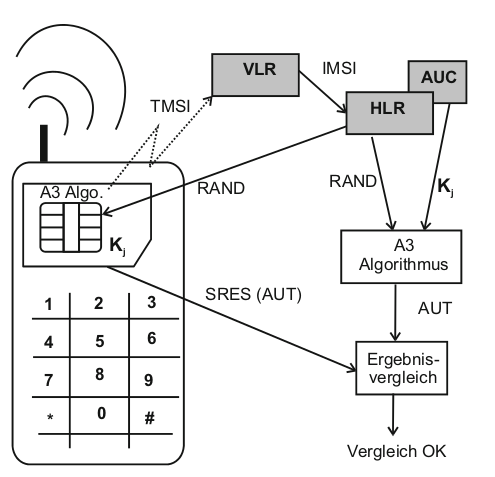
\includegraphics[width=180pt]{simauth_chipkartensicherheit}
 \end{center}
 \caption[Ablauf der GSM-Authentifizierung]{Ablauf der GSM-Authentifizierung \cite{spitz11}}
 \label{abb:simauth}
\end{figure}

Das \ac{HLR} überprüft dann mittels \ac{IMSI} die Benutzerrechte des Teilnehmers und
stößt den Authentifizierungsvorgang an. Selbiger wird dann auf der Seite des
Mobilfunkteilnehmers sowie Providers ausgeführt und das Ergebnis verglichen.
Stimmen beide Ergebnisse überein werden weiterführend Sitzungsschlüssel erzeugt,
mit welchen die Nutzdaten (z.B. Sprache) sicher übertragen werden können.

\paragraph{UMTS} weist einige Unterschiede zum GSM-Mobilfunknetz auf, wobei die
vorhergehende Architektur aus Gründen der Abwärtskompatibilität weiterhin bestehen bleibt
(\ac{VLR},\ac{HLR},\ac{AuC}). Es wird die Variante der USIM als zentrale Chipkarte
eingesetzt. Der Ablauf der Authentifizierung hingegen weicht vom Vorgänger etwas ab.
Dieser wird dadurch erweitert, dass das \ac{AuC} sich nun auch gegenüber der \ac{USIM}
authentifiziert. Auf diesem wird die Sicherheit verbessert, da in beide Richtungen
geprüft wird, ob eine valide Gegenstelle vorliegt. \ac{IMSI}-Catchern wird es damit
schwerer gemacht, eine Form des \textit{Man-In-The-Middle}-Angriffs zu ermöglichen.
Dementsprechend wird auch das Mitschneiden von Gesprächen erschwert. Weiterführend
wird im Gegensatz zu \ac{GSM} nun auch der Verkehr zwischen \ac{HLR} und \ac{VLR}
verschlüsselt realisiert \cite{spitz11}.
Die Authentifizierung selbst über den Milenage-Algorithmus ist ebenfalls ausgebaut
und verfügt nun über weitere Vektoren, die im nachfolgenden Kapitel näher
erläutert werden.

%% Authentifizierungsvorgang %%
\subsection[Authentifizierungsvorgang (Heumann)]{Authentifizierungsvorgang}
\label{authentifizierungsvorgang}

Eine Darstellung des Authentifizierungsvorgangs ist in \Abbildung{kommunikationswege} zu
sehen. Diese beschreibt nur die Authentifizierung einer \ac{USIM}-Karte, aber nicht einer
GSM \ac{SIM}-Karte. \\
Die Authentifizierung ist recht umfangreich und soll hier anhand des Diagramms näher
erläutert werden. Anschließend wird auf die Stärken des Authentifizierungs\-vorgangs
eingegangen unter anderem in Bezug auf die Vorgehensweise in GSM.

 \subsubsection[Ablauf (Heumann)]{Ablauf}
 
 \begin{figure}[htp]
 \begin{center}
  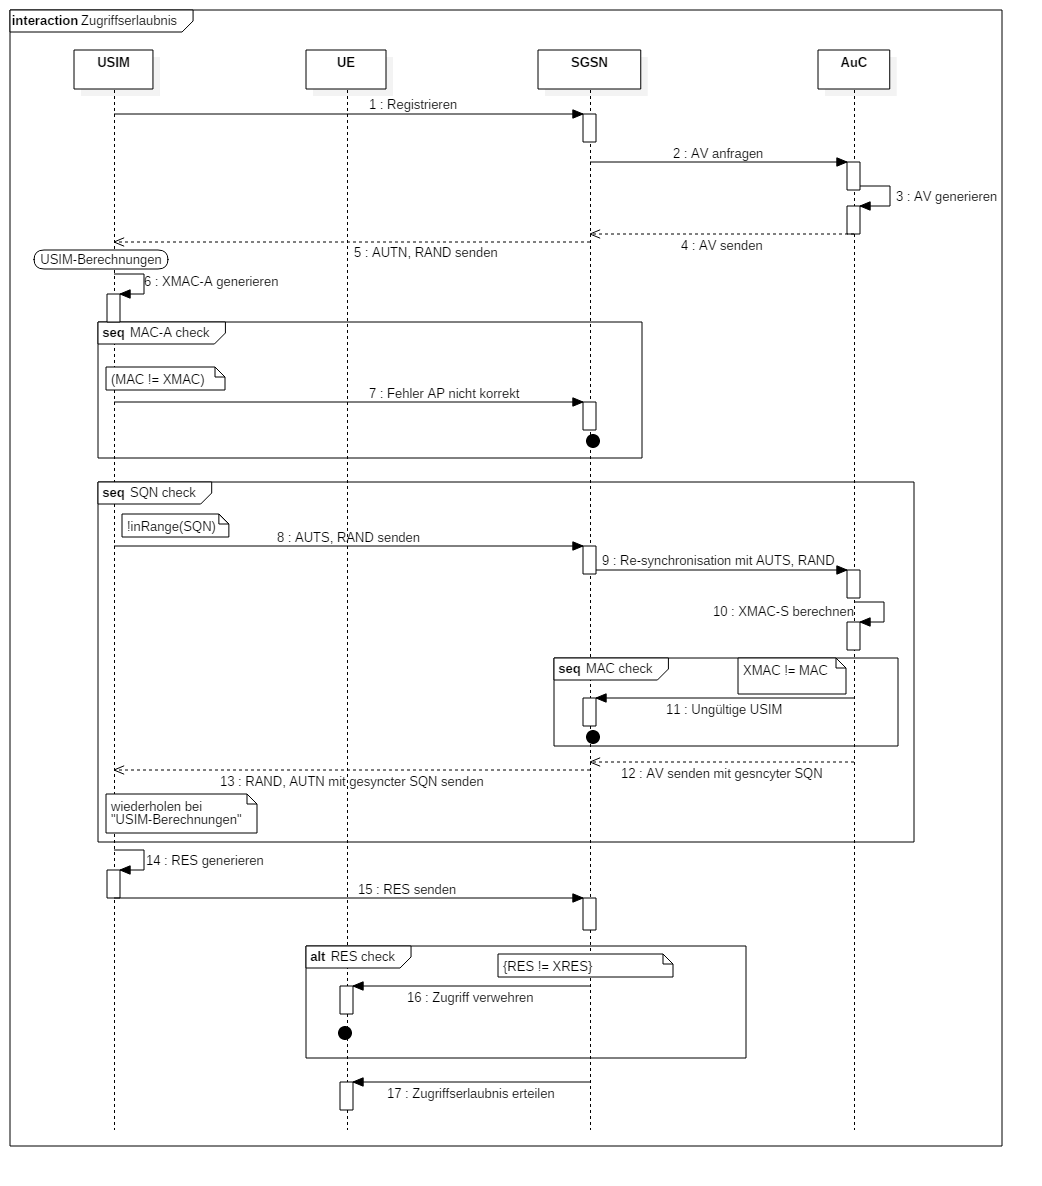
\includegraphics[width=440pt]{kommunikationswege}
 \end{center}
 \caption[Sequenzdiagramm über die Kommunikation zwischen SIM-Karte und Authentication Center]{Sequenzdiagramm über die Kommunikation}
 \label{fig:kommunikationswege}
\end{figure}

 Die Authentifizierung mit \ac{USIM}-Karten geschieht in zwei Richtungen. Es muss nicht nur die
 USIM verifizieren können, dass sie eine valide Karte ist, sondern der Netzprovider muss sich auch
 gegenüber der USIM verifizieren. Möchte eine USIM nun Zugang zum Netz erhalten, schickt sie
 eine Registrierungsanfrage an den nächsten \ac{MSC}. Diese fragt daraufhin beim \ac{AuC} des
 Netzproviders nach einem \ac{AV}. Dieser wird berechnet und nutzt dabei den in Kapitel
 \ref{milenage} auf S. \pageref{milenage} angesprochenen Milenage-Algorithmus. \\
 Der AV ist ein Quintett und besteht aus
 
 \begin{description}
  \item [RAND] Ein Zufallswert, der vom AuC jedes Mal neu generiert wird
  \item [XRES] Der Wert mit dem sich die USIM verifiziert
  \item [CK, IK] Für Verschlüsselungs- und Integritätsschutz bei der späteren Kommunikation
  \item [AUTN] Authentifizierungstoken, den die USIM benötigt. Ist selber ein Triplet aus:
  \begin{description}
   \item [SQN $\oplus$ AK] Eine Sequenznummer verschleiert durch einen Anonymitätsschlüssel
   \item [AMF] Providerspezifisches Managementfeld
   \item [MAC-A] Token zur Verifizierung des Netzwerks
  \end{description}
 \end{description}
 
 Die Werte XRES, CK und IK speichert der MSC zwischen und RAND, sowie AUTN werden an die USIM
 weitergegeben als Antwort auf die Registrierungsanfrage.

 Mit Hilfe des RAND kann die USIM nun den XMAC-A berechnen, also den erwarteten Netzwerktoken, um
 zu überprüfen, ob die USIM sich bei dem richtigen Netzprovider registriert. Wenn XMAC-A
 und MAC-A nicht übereinstimmen, wird dem MSC mitgeteilt, dass die Authentifizierung nicht erfolgreich
 war und die Kommunikation beendet.

 Sollten die Werte jedoch wie erwartet übereinstimmen, überprüft die USIM, ob die SQN im erlaubten
 Bereich ist. Wenn dem nicht so ist, bedeutet das nicht automatisch, dass die Kommunikation wieder
 beendet wird. Die USIM speichert die gültige SQN, was in Kapitel \Verweis{milenage-funktion}
 nochmal näher erläutert wird. Diese wird bei jeder Authentifizierungsanfrage aktualisiert und so kann
 es passieren, dass das AuC keine aktuelle SQN generiert hat und eine Resynchronisation vorgenommen
 werden muss, welche am Ende dieses Kapitels erklärt wird.
 
 Wenn die SQN im erlaubten Bereich liegt, generiert die USIM ihrerseits RES und schickt diesen an
 den MSC. Der MSC überprüft nun, ob XRES des Authenticaton Centers mit dem RES der USIM
 übereinstimmt. Je nach Ergebnis erteilt der MSC dem \ac{UE} den Zutritt zum Mobilfunknetz oder
 nicht.
 
 \paragraph{Resynchronisation}
 \label{par:resynchronisation}
  Wie vorher in diesem Kapitel erwähnt, kann es passieren, dass die SQN zwischen USIM und AuC
  nicht mehr synchron sind und deswegen resynchronisiert werden müssen. Dafür generiert die
  USIM ebenfalls einen RAND-Wert und einen AUTS-Token, welcher dem AUTN sehr ähnlich ist.
  Der AUTS hat im Gegensatz zum AUTN aber keinen AMF und statt dem MAC-A, wird ein MAC-S
  verschickt. Die SQN im AUTS, die geschickt wird, ist die letzte gültige SQN, die die USIM erhalten
  hat. Aus dieser SQN kann das AuC nun eine gültige SQN berechnen. Wichtig ist an dieser
  Stelle zu erwähnen, dass SQN auch bei der Resynchronisation mit einem AK verknüpft wird,
  aber dieser AK wird etwas anders berechnet, als der AK der für die erste SQN seitens des
  Netzproviders verwendet wurde. Genauer wird dies in Kapitel \Verweis{milenage-funktion}
  erklärt.\\
  Ähnlich wie bei der Authentifizierung berechnet diesmal das AuC eine XMAC-S und vergleicht
  diese mit dem MAC-S aus dem AUTS. Sind diese nicht gleich, geht wieder eine Meldung an den
  MSC, der einen Fehler meldet und den Authentifizierungsvorgang beendet. Wenn diese Werte
  jedoch gleich sind, wird mit Hilfe der neuen SQN nochmal der AV berechnet und an den MSC
  geschickt. Dieser gibt wieder AUTN und RAND an die USIM weiter, welche die selben Schritte
  wie zuvor ausführt und diesmal zu dem Ergebnis kommen sollte, dass SQN im erlaubten
  Bereich liegt.
  
  Als Quelle für dieses Kapitel und für weitere Informationen dient \cite{3gpp.33.102}.
  
 \subsubsection[Stärken der UMTS Authentifizierung (Heumann)]{Stärken der UMTS Authentifizierung}
 Der Aufbau der \ac{UMTS}-Struktur beruht auf der selben Struktur, wie bereits \ac{GSM}.
 Denn auch wenn GSM einige Schwächen aufweist, zeigt die zehnjährige Existenz von GSM,
 dass die Sicherheitsarchitektur gut ist \cite{putz01}. Deshalb hat sich die \ac{3GPP} auch
 dazu entschieden, dass die Basis\-sicherheits\-features erhalten bleiben in UMTS. Konkret
 nennen Pütz, Schmitz und Martin (s. \cite{putz01}) unter anderem die folgenden Punkte:
 
 \begin{itemize}
  \item Vertraulichkeit der Teilnehmeridentität
  \item Teilnehmerauthentifizierung gegenüber dem Netzwerk
  \item Authentifizierung des Teilnehmers gegenüber der SIM
  \item Sicherheitsfunktionen ohne Aktion des Nutzers
  \item Eine Authentifizierungsmethode, die vom \ac{SN} durchgeführt wird, aber der gleichzeitig nur minimal vertraut werden muss
  \item Die Möglichkeit für jeden Provider eigene Authentifizierungsalgorithmen zu nutzen
 \end{itemize}
 
 Zusätzlich zu den Sicherheitsfeatures, die aus GSM übernommen wurden, hat UMTS einige
 Schwächen aus GSM beseitigt oder zumindest das Ausnutzen eben jener erschwert. \\
 So können abgefangene \acp{AV} von Angreifern nicht wiederverwendet werden, da
 die SQN eingeführt wurde. \cite{putz01}\\
 Außerdem muss sich nun auch der Netzprovider der USIM gegenüber verifizieren, was
 Man-in-the-Middle Angriffe erschwert. \cite{putz01} \\
 Als letzter Punkt ist zu erwähnen, dass Daten noch länger verschlüsselt bleiben, als noch
 bei GSM, was die Angriffspunkte, an denen man an die unverschlüsselten Daten direkt
 kommt, weiter minimiert. \cite{spitz11}

%% Milenage Algorithmus %%
\subsection[Milenage Algorithmus (Heumann)]{Milenage Algorithmus}
\label{milenage}
Zwischen \ac{SIM}-Karte und Netzprovider muss eine sichere Authentifizierung und
Kommunikation gewährleistet werden können. Dies ist bei dem für den USIM-Vorgänger
entwickelten Algorithmus des \ac{3GPP} nicht
gewährleistet. Mit der Entwicklung des neuen Netzstandards wurde deshalb entschieden,
auch einen neuen Algorithmus zu entwickeln, namentlich der Milenage Algorithmus. \\
Dieser verfügt über die sieben Funktionen \emph{f1}, \emph{f1*}, \emph{f2}, \emph{f3},
\emph{f4}, \emph{f5}, \emph{f5*}, mit Hilfe derer eine sichere Authentifizierung und
Schlüsselgenerierung ermöglicht wird. Die Funktionen mit \emph{*} sind dabei für die
Re-synchonisation nötig, welche im Zuge dieser Arbeit auch durchgeführt wird. \\
3GPP hat, wie auch beim Vorgänger, diese Funktionen nicht näher spezifiziert und ermöglicht
den Netzprovidern eigene Lösungen zu implementieren. Deshalb wird nur beschrieben, in
welchem Kontext diese Funktionen Anwendung finden und generelle Anforderungen
an diese Algorithmen definiert \cite{3gpp.35.205}.

Der Milenage Algorithmus hat wie erwähnt zwei Hauptaufgaben, nämlich einerseits die
Authentifizierung und anderereits die Generierung eines Schlüssel, um die versendeten Nachrichten zu
ver- und entschlüsseln.

In den nachfolgenden Unterkapiteln werden die Vorteile und die Funktionsweise des
Algorithmus, erläutert.

 \subsubsection[Warum Milenage sicher ist (Heumann)]{Warum Milenage sicher ist}
 In Kapitel \Verweis{authentifizierungsvorgang} wurde schon erklärt, dass die Mechanismen
 zur Authentifizierung und zum Schlüsselaustausch angepasst wurden und durch einige
 Änderungen Vorteile mit sich bringen, aber auch der weiterentwickelte Algorithmus zur
 Berechnung der Daten weißt einige Vorteile auf. \\
 Ein wichtiger Punkt dabei ist, dass der Vorgänger geheim war, aber Milenage wurde öffentlich
 diskutiert. Der Vorteil der Offenlegung ist, dass auf diesem Weg Schwachstellen bemerkt werden
 bevor der Algorithmus implementiert ist. 
 
 Stephan Spitz zeigt in seinem Buch ``Kryptographie und IT-Sicherheit'' \cite{spitz11} drei
 wesentliche Gründe auf, die den Algorithmus sicher machen:
 
 \paragraph{Ergebnisse mit hoher Entropie}
 Wenn der Schlüssel K unbekannt ist und die Eingabeparameter \ac{SQN}, RAND
 und \ac{AMF} variieren, dann werden ``sehr gute Pseudo-Zufalls-Ergebnisse mit einer hohen
 Entropie'' \cite{spitz11} erreicht. Dafür muss aber auch eine gute Blockchiffre wie AES
 eingesetzt werden.
 
 \paragraph{Keine Rückschlüsse auf K möglich}
 Wenn die Eingabe- und Ausgabeparameter der einzelnen Funktionen \emph{f1} bis \emph{f5}
 analysiert werden, lassen sich keine Rückschlüsse auf den Schlüssel K oder das \acf{OP}
 ziehen, auch nicht auf Teile dessen. Dies hängt unter anderem damit zusammen, dass K nicht
 direkt in die Funktionen eingeht.
 
 \paragraph{Schlüssellänge}
 Brut-Force-Angriffe, also stumpfes ausprobieren der Schlüssel, dauert aufgrund der
 Schlüssellänge von 128 Bits selbst mit aktuellen Computern noch zu lange.
 
%% TODO #edit bei bedarf hier noch die Vorraussetzungen an die Parameter bzw. wie diese modifiziert werden können

 \subsubsection[Funktionsweise (Heumann)]{Funktionsweise}
 \label{milenage-funktion}
 In Kapitel \Verweis{authentifizierungsvorgang} wurde beschrieben, welche Daten zwischen
 \ac{AuC} und \ac{UE} verschickt, jedoch nicht, wie diese Daten generiert werden. Es
 gibt einige Werte, die auf der \ac{USIM} und der Datenbank des \ac{AuC} fest eingespeichert
 sind. Diese sind der \ac{OP} und K, sowie jeweils fünf Rotations- und XOR-Konstanten
 (r1, ..., r5 und c1, ... c5). Welche Funktion welche Werte benötigt und generiert, zeigt dabei \Abbildung{funktionsubersicht}.
 
 \begin{figure}[htp]
  \begin{center}
   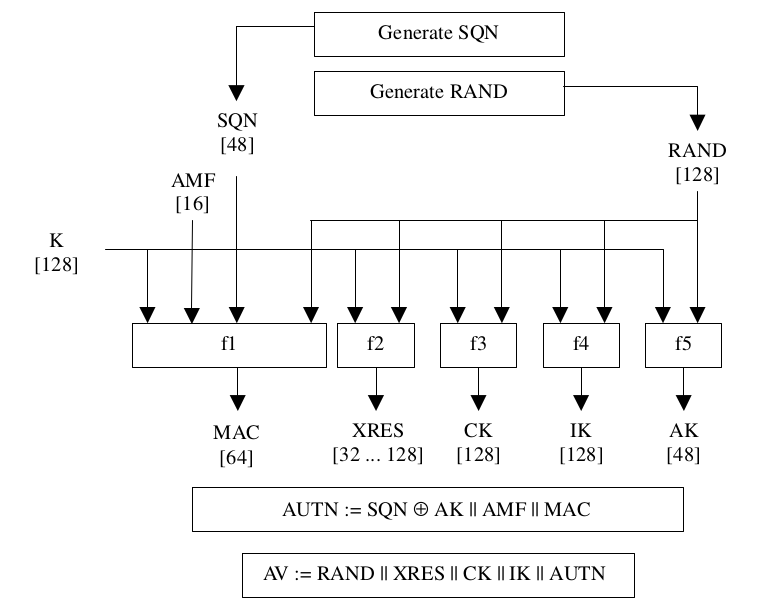
\includegraphics[width=300pt]{generation_of_authentication_vectors}
  \end{center}
  \caption[Übersicht über die Generierung der Authentifizierungsvektoren]{Übersicht über die Generierung der Authentifizierungsvektoren \cite{3gpp.33.102}}
  \label{fig:funktionsubersicht}
 \end{figure}
 
 In \Abbildung{funktionsubersicht} ist zu sehen, dass zu Beginn die \ac{SQN} generiert wird.
 Diese ist insgesamt 48 Bits lang und besteht aus den beiden Teilen SEQ und IND, mit SEQ als
 die eigentliche Sequenznummer und IND als Arrayindex. Dieser Index wird benötigt, da auf
 der SIM-Karte die letzten SQNs in einem Array gespeichert sind. Die empfohlene Arraygröße ist
 32, was für IND eine Länge von fünf Bits bedeutet. Mit diesem Index kann nachher die
 Aktualität der SEQ überprüft werden.\cite{3gpp.33.102} \\
 Für die Bildung der SEQ selbst gibt es drei verschiedene Möglichkeiten:
 \begin{itemize}
  \item teilweise zeitbasiert
  \item nicht zeitbasiert
  \item komplett zeitbasiert
 \end{itemize}
 
 Die einfachste Variante ist die nicht zeitbasierte Lösung, bei der lediglich ein Zähler hochgezählt
 wird mit jeder Authentifizierungsanfrage. Die SEQ ist initial also 0 und wird hochgezählt. Das
 \ac{AuC} speichert in einer Datenbank \cite{3gpp.33.102} zu jeder USIM die aktuelle SQN.
 Auf die anderen  Möglichkeiten wird hier nicht näher eingegangen, da sie in dieser Arbeit
 keine Anwendung finden und deutlich komplexer sind.
 
 Als nächstes wird die RAND gebildet. Das Verfahren, mit dem der Netzprovider diese RAND
 generiert, darf nicht offen gelegt werden, da dies die Sicherheit stark beeinflussen würde. Die
 Spezifikation gibt deshalb für die Generierung der RAND keine Empfehlung, wie für die anderen
 Werte. Generell handelt es sich bei der RAND um eine 128 Bits lange Zufallszahl, die für alle
 anderen Funktionen benötigt wird.
 
 \Abbildung{funktionsubersicht} zeigt zwar, welche Variablen in die Funktionen einfließen und
 welche Werte sie zurückgeben, aber sie zeigt nicht näher, wie diese Werte nun in den einzelnen
 Funktionen angewendet werden. Dies zeigt \Abbildung{schematisch_milenage} besser. Dort ist
 zu erkennen, dass \emph{f2} bis \emph{f5*} nach dem selben Schema berechnet werden können und
 \emph{f1}, sowie \emph{f1*} noch einige zusätzliche Parameter benötigen.
 
 Zunächst die Erklärung der Symbole sowie einiger weiterer Abkürzungen. OPc wird durch
 folgende Formel generiert:
 \begin{center}
  $OP_{C} = OP \oplus E(OP)_{K}$
 \end{center}
 
 $E()$ ist die Blockchiffre. In diesem Fall wird also \ac{OP} mit dem Schlüssel K
 verschlüsselt. Welche Verschlüsselung gewählt wird, gibt 3GPP nicht vor. In
 dieser Arbeit wurde \ac{AES} verwendet, welche im Kapitel \Verweis{aes} näher beschrieben wird. \\
 Der verschlüsselte OP wird dann im zweiten Schritt über XOR ($\oplus$) mit dem ursprünglichen
 OP verknüpft.
 
 \begin{figure}[ht]
  \begin{center}
   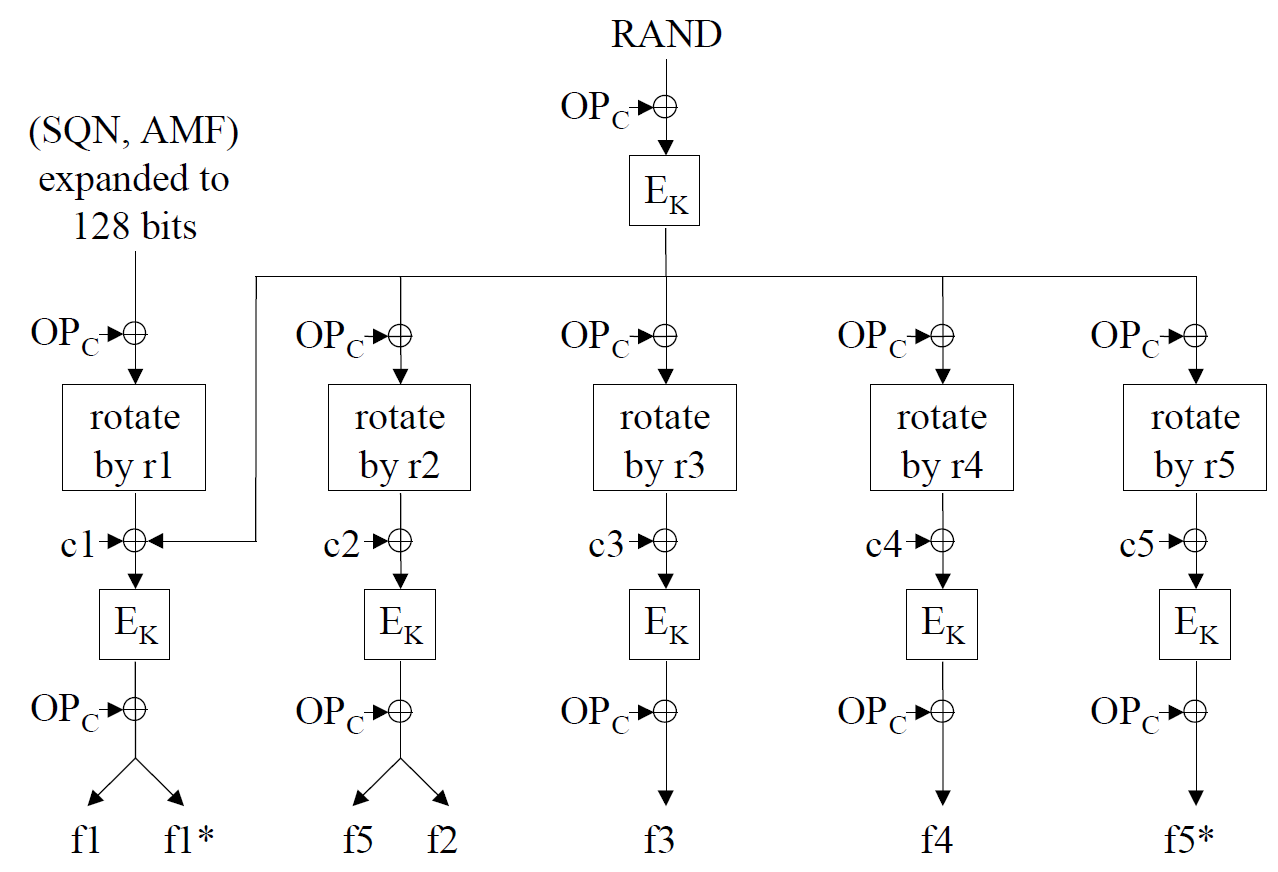
\includegraphics[width=400pt]{detailed_generation_of_authentication_vectors}
  \end{center}
  \caption[Schematische Darstellung der Berechnung der Authentifizierungsvektoren]{Schematische Darstellung der Berechnung \cite{3gpp.33.102}}
  \label{fig:schematisch_milenage}
 \end{figure}
 
 In \Abbildung{schematisch_milenage} ist weiterhin der Funktionsblock ``rotate by r'' zu sehen.
 Beim Rotieren wird der Eingabewert um die Anzahl an Bits des Wertes von r rechts rotiert und
 die Bits, die herausfallen, links wieder eingefügt. Beispielsweise wird aus 110101 bei einem
 Rotationswert r von 2: 011101.
 
 Mit den genannten Infos ist verständlich, dass die Funktionen \emph{f2} bis \emph{f5*}
von einem verschlüsselten $RAND \oplus OP_C$ ausgehen, welcher in der Dokumentation
 auch als TEMP bezeichnet wird. Dieser Wert wird wieder über XOR-mit $OP_ C$ verknüpft
 und um die entsprechende Rotationskonstante r rotiert. Im Anschluss wird wieder eine XOR
 Verknüpfung mit der speziellen XOR-Konstante c und die Chiffre des Ausgabewertes durchgeführt. Im
 letzten Schritt wird dieser dann nochmal über XOR mit $OP_{C}$ verknüpft. \\
 Wie die \Abbildung{schematisch_milenage} zeigt, funktionieren \emph{f1} und {f1*} sehr
 ähnlich. Bevor jedoch TEMP in die Berechnung einfließt, wird SQN und AMF auf 128 Bits
 erweitert und bekommt in der Dokumentation die Bezeichnung IN1. IN1 besteht aus SQN und
 AMF abwechselnd konkateniert, also SQN $\|$ AMF $\|$ SQN $\|$ AMF. \cite{3gpp.33.102}
 
 Wie im Kapitel \ref{aes} erklärt wird, sind die Blöcke, die verschlüsselt werden, immer
 128 Bits lang. Das gilt auch für RAND, TEMP oder IN1. Ein MAC-A oder RES
 jedoch sind kürzer, weshalb diese nur aus Teilen eines Blocks bestehen. Deswegen steht
 an manchen Enden des Diagramms in \Abbildung{schematisch_milenage} auch mehr als ein
 Funktionsname. \\
 Es gibt fünf Blöcke, aus denen sich die sieben Funktionswerte bilden. Sie werden in der
 Spezifikation von Milenage mit OUT\emph{n} bezeichnet.
 
 \begin{description}
  \item [OUT1] Beinhaltet die beiden jeweils 64 Bits langen Werte MAC-A und MAC-S
  \item [OUT2] Die ersten 64 Bits sind AK und die hinteren 64 Bits RES
  \item [OUT3] Da CK 128 Bits lang ist, ist OUT3 komplett CK
  \item [OUT4] Ähnlich CK ist auch IK 128 Bits lang
  \item [OUT5] Die ersten 64 Bits sind AK und der Rest wird nicht benötigt
 \end{description}
 
 Es ist kein Fehler, dass AK sowohl bei OUT2 als auch bei OUT5 erwähnt wird, sondern
 wie schon in Kapitel \Verweis{authentifizierungsvorgang} beschrieben, wird
 der Anonymitätsschlüssel AK, der mit SQN verknüpft wird, im Falle der Resynchronisation
 anders berechnet als bei der Generierung der Authentifizierungsvektoren seitens des
 Netzproviders.
 
%% AES/Rijndael %%
\subsection[AES / Rijndael (Heumann \& Schenkel)]{AES / Rijndael}
\label{aes}
 Rijndael oder \ac{AES} sind beides Blockverschlüsselungen. Das bedeutet, dass der zu
 verschlüsselnde Text in gleich große Blöcke aufgeteilt wird und jeder Block mit einem Schlüssel
 chiffriert wird. Die Blocklänge des verschlüsselten Textes bleibt dabei gleich. \\
 Der Unterschied zwischen Rijndael und AES besteht lediglich in der Länge der Text- sowie
 Schlüsselblöcke und ist sonst identisch. Für Rijndael gilt, dass Block- und Schlüssellänge
 unabhängig von einander auf Vielfache von 32 Bits definiert werden können. Minimal müssen
 beide aber 128 Bits lang sein und maximal 256 Bits \cite{daemon02}. \\ %TODO: #edit quelle? #CHECK
 AES auf der anderen Seite hat die Blocklänge auf 128 Bits festgelegt und die Schlüssel\-länge
 darf nur 128, 192 oder 256 Bits betragen \cite{AES-FIPS}. Welche Schlüssel\-länge genutzt
 wird, kann durch die unterschiedlichen Bezeichnung AES-128, AES-192 und AES-256 deutlich gemacht
 werden.
 
 Im folgenden soll kurz die Geschichte von AES beziehungsweise Rijndael erläutert werden und
 wie der Verschlüsselungs\-algorithmus der beiden funktioniert. Nicht angesprochen wird der
 Entschlüsselungs\-algorithmus, da er für diese Arbeit keine Relevanz hat.
 
 \subsubsection[Geschichte (Heumann)]{Geschichte}
 \label{aes-geschichte}
 Die erste Blockverschlüsselung, die vom \ac{NIST} 1977 offiziell übernommen wurde, war
 \ac{DES} und basierte auf einer überarbeiteten Version der Blockverschlüsselung Lucifer. Bei
 DES betrug die Blockgröße nur 64 Bits, was lange Zeit ausreichend war, aber mit Fortschreiten
 der Rechenleistungen nicht mehr lange genügen würde gegen Brute-Force Angriffe (weitere
 Argumente finden sich in \cite{paar10}). Es gab deswegen die Empfehlung, den dreifach DES zu
 nutzen, aber der war nochmal langsamer als der einfache DES, weshalb das NIST eine neue
 Blockverschlüsselung suchte über eine Ausschreibung (1997).
 
 An die neue Verschlüsselung wurden folgende Bedingungen gestellt:
\begin{itemize}
 \item Blockverschlüsselung mit einer Blocklänge von 128 Bits
 \item Die drei Schlüssellängen 128, 192 und 256 Bits müssen unterstützt werden
 \item Sicherheitslevel ähnlich anderer Algorithmen
 \item Effizient in Soft- und Hardware
\end{itemize} 

Die Suche nach dem neuen Algorithmus fand öffentlich statt, sodass sich jeder auf der ganzen
Welt beteiligen konnte und im August 1999 fünf Finalisten gekürt wurden. Dabei wurden
öffentlich die Vor- und Nachteile der einzelnen Algorithmen diskutiert und Ende 2000 gab NIST
mit Rijndael den Gewinner bekannt. Dieser wurde von den beiden Belgiern Joan
Daemon und Vincent Rijmen entwickelt.

An dieser Stelle sei auch erwähnt, dass die \ac{NSA} sehr viel Vertrauen in AES hat. So erteilte
sie diesem die generelle Erlaubnis, als \emph{SECRET} eingestufte Dokumente mit AES zu
verschlüsseln und selbst als \emph{TOP SECRET} eingestufte Dokumente dürfen mit einer
Schlüssellänge von 192 oder 256Bits verschlüsselt werden. \cite{paar10}
 
 \subsubsection[Mitbewerber (Heumann)]{Mitbewerber}
 Als die größten Konkurrenten von Rijndael werden ``Twofish'' und ``Serpent'' gesehen. Um zu verstehen,
 warum die Entscheidung am Ende trotzdem auf Rijndael fiel, sollen die beiden Konkurrenten an dieser
 Stelle untersucht werden. Beide verfolgen einen klassischen Ansatz.
 
 \paragraph{Serpent}
 Entwickelt wurde der Algorithmus von drei bekannten Kyrptografen. Sie haben bei der Entwicklung ihres
 Algorithmus darauf geachtet, dass er noch in mindestens einem Jahrhundert sicher ist und deswegen auch
 auf Experimente verzichtet. Serpent ist wie AES eine Substitutions-Permutations-Chiffre. Sie nutzt
 hauptsächlich Substitutionsboxen und einige lineare Funktionen, welche
 in der Kombination seit den siebziger Jahren bekannt sind und deshalb als gut erforscht gelten.
 Außerdem nutzen sie 32, statt, wie in anderen Verfahren, die üblichen acht bis 16 Runden, um sicher zu gehen. \\
 Serpent hat nach aktuellem Stand einen sehr großen Sicherheitspuffer, da 32 Runden verwendet werden, aber
 diese hohe Anzahl macht ihn auch zu dem langsamsten der Algorithmen. \cite{schmeh07}
 
 \paragraph{Twofish}
 Der Nachfolger von Blowfish ist Twofish, entwickelt unter anderem von Bruce Schneider. Es handelt sich dabei um eine Feistel-Chiffre.
 In Twofish werden vier S-Boxen aus dem
 Schlüssel generiert, die jeweils zwei mal pro Runde eingesetzt werden. Insgesamt sieht Twofish 16 Runden vor.
 Wie auch bei Serpent sind abgesehen von den Substitutionsboxen alle Schritte linear. Es werden insgesamt 40
 Subschlüssel je 32 Bits Länge benötigt und die S-Boxen müssen generiert werden. \\
 Daraus folgt, dass Twofish mit seiner Geschwindigkeit zwischen Rijndael und Serpent liegt. Auch was die Innovationen
 im Design angeht, liegt Twofish zwischen Serpent und Rijndael. Bislang ist nur eine theoretische Schwachstelle
 bekannt, aber keine konkrete Methode, diese zu nutzen. \cite{schmeh07}
 
 \subsubsection[Algebraische endliche Körper (Heumann)]{Algebraische endliche Körper}
 Der Algorithmus ist verständlich und anwendbar, auch ohne das Wissen über die mathematischen
 Grundlagen dazu. Trotzdem beruht die Tatsache, dass der Algorithmus funktioniert, auf Mathematik
 und diese soll hier erläutert werden. Konkret liegt dem Algorithmus die algebraische Struktur des
 endlichen Körpers, auch Galois-Feld genannt, zu Grunde. Doch bevor der endliche Körper
 erklärt werden kann, muss als Basis die algebraische Gruppe definiert werden.
 
 Eine Gruppe ist eine Menge von Elementen $G$ und eine Operation $\circ$, die zwei Elemente
 aus $G$ miteinander kombiniert. Es gelten dabei folgende fünf Eigenschaften für die Gruppe \cite{paar10}:
 
 \begin{enumerate}
 	\item Die Gruppenoperation $\circ$ ist abgeschlossen: $\forall a, b \in G: a \circ b = c \in G$
	\item Die Gruppenoperation ist assoziativ: $\forall a, b, c \in G: a \circ (b \circ c) = (a \circ b) \circ c$
	\item Es gibt ein neutrales Element $e$: $\forall a \in G: a \circ e = e \circ a = a$
	\item Für jedes Element $a$ existiert ein inverses Element $a^{-1}$: $\forall a \in G: a \circ a^{-1} = a^{-1} \circ a = e$
	\item Eine Gruppe ist außerdem kommutativ, wenn $\forall a, b \in G: a\circ b = b \circ a$
 \end{enumerate}

 Als Beispiel sei die Menge $\Z$, mit der Operation $+$ und dem neutralen Element $0$ genannt.
 Dies ist eine kommutative Gruppe mit dem inversen Element $-a$, denn $\forall a \in \Z: a + (-a) = 0$.
 Mit der Operation $*$ hingegen gibt es kein neutrales Element, welches eine Gruppe ermöglichen
 würde. \\
 Anzumerken ist, dass die Menge nicht wie $\Z$ unendlich sein muss, damit eine Gruppenbildung
 möglich ist. Ein Beispiel dafür wird zu einem späteren Zeitpunkt geliefert.
 
 Die Fortsetzung der Gruppe ist der Körper. Diese Struktur unterstützt die vier arithmetischen Basisoperationen
 Addition, Subtraktion, Multiplikation und Division. Die Definition für einen Körper $K$ lautet \cite{paar10}:

 \begin{enumerate}
 	\item Alle Elemente aus $K$ bilden eine additive Gruppe mit dem Gruppenoperator ``$+$'' und dem neutralen Element 0.
	\item Alle Elemente aus $K$, außer 0, bilden eine multiplikative Gruppe mit dem Operator ``$\times$'' und dem neutralen Element 1.
	\item Wenn beide Gruppenoperatoren gemischt werden, gilt das Distributivgesetz: \\
		$\forall a, b, c \in K: a \times (b + c) = (a \times b) + (a \times c)$
 \end{enumerate}

 Ähnlich wie bei Rijndael spielen im Großteil der Kryptographie die endlichen Körper, oder Galois-Feld genannt,
 eine große Rolle. Die endliche Menge, die einen Körper zu einem endlichen Körper macht, ist zählbar und
 die Anzahl der Elemente wird ``Ordnung'' oder ``Kardinalität'' genannt. Ein Körper kann jedoch nur
 mit folgendem Theorem endlich sein \cite{paar10}:
 
 \begin{center}
  \parbox{12cm}{\centering
   Ein Körper mit einer Ordnung $m$ existiert nur, wenn $m$ eine Primzahlpotenz ist:
   $m = p^n$, mit einer positiven ganzen Zahl $n$ und einer Primzahl $p$. $p$ heißt ``Charakteristik''
   von $K$.
  }
 \end{center} 
 
 Daraus folgt, dass ein endlicher Körper mit der Kardinalität von $11 = 11^1$ oder $81 = 3^4$ existiert, aber
 nicht 12, da $12 = 2^2 * 3$. Die einfachsten Körper sind dabei wohl die mit einer Primzahlcharakteristik, also
 mit $n = 1$, sogenannte ``Primkörper''.
 
 Die Elemente des Galois-Felds $GF(p)$ werden mit ganzen Zahlen repräsentiert: $0, 1, \dots, p-1$. Die arithmetischen
 Rechenoperationen werden \emph{modulo} $p$ betrieben. Dadurch ist das additive Inverse eines Elements $a$ gegeben
 mit $a + (-a) = 0$ modulo $p$ und das multiplikative Inverse jedes Elements $a$ außer 0 ist definiert als $a * a^{-1} = 1$.
 Nachfolgend gibt es ein kleines Beispiel mit $GF(5)$ zum besseren Verständnis:
 
 %%TODO: Kriege es nicht besser gestylt...
\begin{minipage}{0.5\textwidth}
\textbf{Addition:} \\ \\
    \begin{tabular}{l|lllll}
    $+$ & 0 & 1 & 2 & 3 & 4 \\ \hline
    0      & 0 & 1 & 2 & 3 & 4 \\
    1      & 1 & 2 & 3 & 4 & 0 \\
    2      & 2 & 3 & 4 & 0 & 1 \\
    3      & 3 & 4 & 0 & 1 & 2 \\
    4      & 4 & 0 & 1 & 2 & 3 \\
    \end{tabular}
    \\
    \\
\end{minipage}
\begin{minipage}{0.5\textwidth}
\textbf{Additives Inverses:}
  \begin{flalign*}
    -0 = 0 \\
    -1 = 4 \\
    -2 = 3 \\
    -3 = 2 \\
    -4 = 1 \\
  \end{flalign*}
\end{minipage}
\begin{minipage}{0.5\textwidth}
\textbf{Multiplikation:} \\ \\
    \begin{tabular}{l|lllll}
    $\times$ & 0 & 1 & 2 & 3 & 4 \\ \hline
    0 	        & 0 & 0 & 0 & 0 & 0 \\
    1             & 0 & 1 & 2 & 3 & 4 \\
    2             & 0 & 2 & 4 & 1 & 3 \\
    3             & 0 & 3 & 1 & 4 & 2 \\
    4             & 0 & 4 & 3 & 2 & 1 \\
    \end{tabular}
    \\
    \\
\end{minipage}
\begin{minipage}{0.5\textwidth}
\textbf{Multiplikatives Inverses:}
  \begin{flalign*}
    0^{-1} &~ \text{existiert nicht} \\
    1^{-1} &= 1 \\
    2^{-1} &= 3 \\
    3^{-1} &= 2 \\
    4^{-1} &= 4 \\
  \end{flalign*}
\end{minipage}
 Ein wichtiger Primkörper ist $GF(2)$, welcher der kleinste endliche Körper ist, der existiert und wichtig
 für AES ist. Die Addition kommt in diesem Körper der booleschen XOR-Operation gleich. Gleichzeitig
 produziert die Multiplikation das selbe Ergebnis wie die boolesche Und-Operation:
 
 \begin{minipage}{0.5\textwidth}
\textbf{Addition:} \\
    \begin{tabular}{l|lllll}
    $+$  & 0 & 1 \\ \hline
    0 	  & 0 & 1 \\
    1       & 1 & 0 \\
    \end{tabular}
    \\
    \\
\end{minipage}
\begin{minipage}{0.5\textwidth}
\textbf{Multiplikation:} \\
    \begin{tabular}{l|lllll}
    $\times$ & 0 & 1 \\ \hline
    0 	        & 0 & 0 \\
    1             & 0 & 1 \\
    \end{tabular}
    \\
    \\
\end{minipage}
 
 Als letzte Struktur sei die Körpererweiterung erwähnt, welche als $GF(2^m)$ geschrieben werden kann,
 mit $m > 1$. AES hat seinen Algorithmus auf der Körpererweiterung $GF(2^8)$ aufgebaut, da sich damit
 alle 256 Werte eines Bytes repräsentieren lassen. Da 256 offensichtlich keine Primzahl ist, können die
 Additionen und Multiplikationen nicht repräsentiert werden durch die Ganzzahlige Addition und Multiplikation
 modulo $2^8$. Deshalb wird zum einen eine andere Notation für die Elemente des Körpers benötigt und
 zum anderen neue Regeln für die Durchführung der arithmetischen Rechenoperationen. Nachfolgend soll
 aufgezeigt werden, dass die Elemente als ``Polynome'' dargestellt werden können und darauf aufbauend
 ``polynome Arithmetik'' durchgeführt werden kann \cite{paar10}. Jedes Polynom $A \in GF(2^m)$ wird
 dargestellt als:
 \begin{equation*}
   A(x) = a_{m-1}x^{m-1} + \hdots + a_1x + a_0, ~~~ a_i \in GF(2)
 \end{equation*}
 
 Die polynome Arithmetik wird nun im folgenden Kapitel speziell für die Körpererweiterung
 $GF(2^8)$ erklärt.
 
 \subsubsection[Polynome Arithmetik in $GF(2^8)$ (Heumann)]{Polynome Arithmetik in $\mathbf{GF(2^8)}$}
 \label{polynome-arithmetic}
 Die Addition bei einem endlichen Körper wird erreicht durch die Addition der einzelnen Koeffizienten. Wie
 im vorherigen Kapitel gezeigt, bedeutet das, dass die jeweiligen Koeffizienten über eine XOR-Operation
 verrechnet werden. Die Addition ist wie folgt definiert \cite{paar10}:
 
 \begin{center}
  \parbox{14cm}{\centering
   Sei $A(x), B(x) \in GF(2^8)$, dann wird die Summe dieser wie folgt berechnet:
   \begin{equation*}
    C(x) = A(x) + B(x) = \sum_{i=0}^7 c_ix^i, ~~~ c_i \equiv a_i + b_i ~\text{mod}~ 2
   \end{equation*}
  }
 \end{center} 
 
 Nachfolgend ist ein kurzes Beispiel der Addition mit unterschiedlichen Notationen
 aufgeführt:
 
 \begin{equation}
  \begin{aligned}
   (x^6 + x^4 +x^2 + x + 1) + (x^7 + x + 1) &= x^7 + x^6 + x^4 + x^2 & \text{(polynome Notation)} &\\
   01010111_2 \oplus 10000011_2 &= 11010100_2 & \text{(binäre Notation)} &\\
   57_{16} \oplus 83_{16} &= d4_{16} & \text{(hexadezimale Notation)} &\\
  \end{aligned}
  \label{math:addition}
 \end{equation}
 
 In der polynomen Repräsentation entspricht die Multiplikation in $GF(2^8)$ (dargestellt durch $\cdot$) der
 Multiplikation von Polynomen modulo eines ``irreduziblen Polynoms'' achten Grades. Dabei ist ein Polynom
 irreduzibel, wenn es nur durch 1 und sich selbst teilbar ist ähnlich einer Primzahl. Das irreduzible
 Polynom des AES-Algorithmus lautet:
  \begin{equation}
   m(x) = x^8 + x^4 + x^3 + x + 1
  \label{math:aes-polynom}
  \end{equation}
 Ein Beispiel eines reduzierbaren Polynoms ist $x^8 +x^3 + x^2 + 1$, da
 \begin{equation*}
   x^8 +x^3 + x^2 + 1 = (x^5 + x^2 + 1) \cdot (x^3 + 1)
 \end{equation*}
 
 Mit der Kenntnis des irreduziblen Polynoms lässt sich auch die Multiplikation vollständig definieren:
 
 \begin{center}
  \parbox{13cm}{\centering
   Sei $A(x), B(x) \in GF(2^8)$, dann wird die Multiplikation von zwei Elementen $A(x), B(x)$
   und irreduziblen Polynom $m(x)$ berechnet mit
   \begin{equation*}
    C(x) = A(x) \cdot B(x) ~\text{mod}~ m(x)
   \end{equation*}
  }
 \end{center} 
 
 So ist bei der Multiplikation statt Addition der beiden Polynome aus Gleichung \ref{math:addition} das
 Ergebnis $x^7 + x^6 +1$.
 
 Das Multiplizieren zweier Polynome auf dem einfachsten Weg ohne Tricks dauert jedoch ziemlich lange
 und im Anschluss muss noch durch $m(x)$ dividiert werden. Das führt zwar am Ende zum richtigen Ergebnis,
 aber ist, wie gesagt, sehr zeitaufwändig. In der Spezifikation des AES wird deshalb eine Methode angeboten,
 mit der ebenfalls das richtige Ergebnis zustande kommt, aber wesentlich effizienter.
 
 Die Funktion, die in der Spezifikation vorgeschlagen wird, heißt \emph{xtime(A(x))} und multipliziert
 $A(x)$ mit $x$ und reduziert durch $m(x)$. Es gilt:
 \begin{equation*}
    C(x) = xtime(A(x)) = A(x) * x = \sum_{i=0}^7 a_ix^{i+1}, ~ \text{für}~ A \in GF(2^8)
 \end{equation*}
 
 Um bei einer Größe von 8 Bits für $C(x)$ zu bleiben, wird vor der Schiebeoperation überprüft, ob
 $a_7$ 0 oder 1 ist. Wenn das Bit 0 ist, wird nach Anwendung der Funktion $C(x)$ kleiner $m(x)$ sein. In
 diesem Falle ist im Anschluss keine Modulo-Operation notwendig. Diese wird nur erforderlich, wenn $a_7$ 1 ist. Dann
 muss C(x) noch modulo dem hinteren Teil von $m(x)$ berechnet werden, nämlich $x^4 + x^3 + x +1$. Es
 muss nur mit dem hinteren Teil des irreduziblen Polynom $m(x)$ reduziert werden, da $x^8$ nicht genutzt
 wird in $C(x)$. \cite{AES-FIPS}
 
 Weiter ist $C(x) = m(x) + r$, wobei $r = A(x)$ mod $m(x)$. Daraus folgt:
 \begin{equation*}
    C(x) = xtime(A(x)) \oplus \begin{cases}
      0	 		& \text{wenn $a_7 = 0$},\\
      00011011_2 	& \text{wenn $a_7 = 1$}.
     \end{cases}
 \end{equation*}
 
 Die Funktion \emph{xtime()} kann außerdem rekursiv verwendet werden. Das bedeutet, dass
 \begin{equation*}
    A(x) * x^3 = xtime(A(x) * x^2) = xtime(xtime(A(x) * x)) = xtime(xtime(xtime(A(x))))
 \end{equation*}
 
 Das Ergebnis der Berechnung zweier Werte $A(x), B(x)$ kann dadurch erzielt werden, dass die einzelnen
 Zwischenergebnisse von $B(x)$ aufaddiert werden mit $A(x)$. Dazu ein letztes Beispiel:
  \begin{flalign*}
   &A(x) = x^6 + x^4 + x^2 + x^1 + 1, B(x) = x^4 + x^1 + 1 \\
   &A(x) \cdot B(x) = x^7 + x^6 + x^5 + x^4 + x^3 + x^2 + x^1 ~~\text{, weil} \\
   &A(x) * x^1 = x^7 + x^5 + x^3 + x^2 + x^1 \\
   &A(x) * x^4 = x^2 + x^1 + 1 \\
   &\Rightarrow ( x^6 + x^4 + x^2 + x^1 + 1) \oplus (x^7 + x^5 + x^3 + x^2 + x^1) \oplus (x^2 + x^1 + 1) \\
   %TODO: #edit Eine bessere Idee zur Formatierung wäre gut
   & ~~~~~~~~~~~~~~~~~~~~~~~~~~~~~~~~~~~~~~~~~~~~~~~~~~~~~~~~~~~~~~ = x^7 + x^6 + x^5 + x^4 + x^3 + x^2 + x^1 \\
  \end{flalign*}
 
 Damit ist die Berechnung der beiden Elemente deutlich effizienter und dient als gute Grundlage für die
 Implementierung der AES-Chiffre. Diese wird im folgenden Kapitel beschrieben.
 
 \subsubsection[Funktionsweise (Heumann)]{Funktionsweise}
 \label{aes-funktion}
 Bei der Blockverschlüsselung gibt es fünf verschiedene Betriebsmodi, die in der ISO/IEC 10116:2006
 \cite{ISO10116} beschrieben sind. Diese Betriebsmodi geben an, wie ein Text bestehend aus
 mehreren Blöcken verschlüsselt wird.
 
  \paragraph{Electronic Codeblock (ECB)}
   Jeder Textblock wird unabhängig vom vorherigen Block verschlüsselt. Daraus resultieren vor allem
   zwei Dinge. Zum einen führt eine Vertauschung der Blöcke im chiffrierten Text zur gleichen Vertauschung
   im entschlüsselten Text und zum anderen beeinflusst ein Fehler bei der Entschlüsselung eines Blocks
   nicht die anderen Blöcke. Es wird deshalb davon abgeraten, diesen Modus zu verwenden bei mehr
   als einem Block.

  \paragraph{Cipher Block Chaining (CBC)}
   Beim CBC werden die Schwächen von ECB verkleinert, in dem eine Verkettung der Blöcke vorgenommen
   wird. So gibt es beim ersten Block zusätzlich zum Schlüssel noch einen Initialisierungsvektor. Bei den
   folgenden Textblöcken wird der Schlüssel mit dem vorhergehenden verschlüsselten Textblock
   verknüpft. Dadurch können Blöcke nicht mehr vertauscht werden und wenn ein Fehler bei der Entschlüsselung
   in einem Block entsteht, ist zusätzlich zu diesem auch der nachfolgende Block nicht mehr
   zu entschlüsseln.
   
  Neben den beiden genannten Modi existieren noch ``Cipher Feedback'', ``Output Feedback'' und
  ``Counter''. Auf diese soll hier aber nicht näher eingegangen werden, da diese Elemente die
  Stromchiffre nutzen. Ihre Erklärung wäre deshalb in diesen Rahmen zu umfangreich, da beim
  Mileange-Algorithmus nur Zeichenketten verschlüsselt werde, die nicht länger oder kürzer als ein Block
  sind. Das ist auch der Grund, warum bei Milenage bedenkenlos der ECB eingesetzt werden kann.
  
  Beim AES-Algorithmus werden nicht nur Teile sondern immer alle 128 Bits bearbeitet, weshalb die
  Anzahl der Iterationen relativ gering ist und den Algorithmus schnell machen. Bei einer Schlüssellänge
  von 128 Bits werden 10 Runden benötigt, bei 192 Bits 12 und bei der Schlüssellänge von 256 Bits
  sind 14 Runden nötig. In jeder Runde werden vier Funktionen auf den Textblock angewendet, um
  ihn gut zu verschlüsseln. In welcher Reihenfolge diese angewendet werden, wird später
  in diesem Kapitel erläutert.
  
  Damit der Textblock mit einem Schlüssel verschlüsselt werden kann, müssen beide in ein rechteckiges
  Array aus Bytes transformiert werden. Die Anzahl der Reihen ist immer vier, aber die Anzahl der Spalten
  variiert je nach Textlänge. Mit der Umwandlung des Textblocks in das Array spricht man vom Zustand
  und der umgewandelte Schlüssel ist nun der Chiffrierschlüssel. \\
  Der Zustand ist bei AES immer vier Spalten und der Chiffrierschlüssel vier, sechs oder acht Spalten
  breit. In beiden Fällen wird das Array zeilenweise gebildet. Das bedeutet, dass bei einer Blocklänge von
  128 Bits in den ersten vier Arrayelementen des Zustands die ersten 32 Bits des Blocks stehen.
  
  Nachfolgend werden nun die vier Funktionen beschrieben, die den Zustand verändern.
  
  \paragraph{SubBytes}
   Bei der SubBytes-Transformation handelt es sich um eine nicht-lineare Bytesubstitution, welche
   separat auf jedes Byte des Status angewendet wird. Die Substitutionstabelle, auch S-Box genannt,
   ist 16 x 16 Felder groß und damit eine bijektive Abbildung aller 256 möglichen Eingabemöglichkeiten.
   Wie die Tabelle gebildet wird, wird an dieser Stelle nicht näher beschrieben aber im \Anhang{abb:s-box}
   befindet sich die Tabelle.
   
   Mit dem Wert das Statuselements wird nun der Wert aus der Substitutionstabelle ermittelt. Die ersten vier
   Bits geben die Zeile vor und die letzten viert Bits die Spalte. So wird beispielsweise der Wert $8D_{16}$ mit
   $5D_{16}$ substituiert.
   
  \paragraph{ShiftRows}
   Bei dieser Funktion werden die Bytes in jeder Zeile des Zustands-Arrays zirkulär verschoben. Das bedeutet,
   dass die einzelnen Bytes vorne, also links, ``rausgeschoben'' werden und hinten/rechts, wieder
   ``reingeschoben''. Dabei ist  die Anzahl der Verschiebungen in jeder Zeile unterschiedlich. In Zeile eins wird
   das Array gar nicht verschoben, in Zeile zwei um ein Byte, Zeile drei um zwei Bytes und in Zeile vier um drei
   Bytes. Für die Berechnung existiert keine mathematische Grundlage, sondern es geht einfach
   um die Konfusion des Arrays.
   
   Als Beispiel sei der String in der vierten Zeile $3B | 2A | 34 | 71$, so würde dieser durch die Rotation anschließend
   so aussehen: $71 | 3B | 2A | 34$.
   
  \paragraph{MixColumns}
   In der MixColumns-Transformation wird nicht jedes Byte einzeln transformiert, sondern die gesamte Spalte.
   Die Berechnung ist hierbei etwas umfangreicher als in den Transformationen zuvor. Nehmen wir eine Spalte
   $j$, dann wird folgende Berechnung durchgeführt:
   
    \begin{equation*}
     \begin{split}
     b_{0,j} = T_2(a_{0,j}) \oplus T_3(a_{1,j}) \oplus a_{2,j} \oplus a_{3,j} \\
     b_{1,j} = a_{0,j} \oplus T_2(a_{1,j}) \oplus T_3(a_{2,j}) \oplus a_{3,j} \\
     b_{2,j} = a_{0,j} \oplus a_{1,j} \oplus T_2(a_{2,j}) \oplus T_3(a_{3,j}) \\
     b_{3,j} = T_3(a_{0,j}) \oplus a_{1,j} \oplus a_{2,j} \oplus T_2(a_{3,j})
     \end{split}
    \end{equation*}
    
    $T_2(a)$ ist nun definiert als:
    
    \begin{equation*}
     \begin{aligned}
     T_2(a) = \begin{cases}
      2 * a 		 & \text{wenn $a < 128$},\\
      (2*a) \oplus 283 & \text{wenn $a \geq 128$}.
     \end{cases}
     \end{aligned}
    \end{equation*}
    
    Die Definition von $T_3(a)$ ist lediglich $T_2(a) \oplus a$.
    
    Durch diese Definition gilt, dass wenn $a = 143$, dann
    \begin{equation*}
     \begin{aligned}
     T_2(143) &= 5 \\
     T_3(143) &= T_2(143) \oplus 143 = 138
     \end{aligned}
    \end{equation*}
    
    Mathematisch betrachtet beruht diese Funktion auf Polynomen mit Koeffizienten aus $GF(2^8)$. Statt also
    Koeffizienten, die ein Bit repräsentieren, repräsentiert in diesem Fall ein Koeffizient ein ganzes Byte. Für diese
    Polynome kann gezeigt werden, dass die Funktion $T_2(a)$ auch beschrieben werden kann als $2 \cdot a$.
    Ähnliches gilt für $T_3(a)$ mit $3 \cdot a$ \cite{schmeh07}.
   
  \paragraph{AddRoundKey}
   In dieser Funktion wird jedes einzelne Zustandsbyte mit einem Byte aus dem Rundenschlüssel bitweise über
   ein exklusives Oder verrechnet. Der Rundenschlüssel ist ein erweiterter Chiffrierschlüssel. Die Berechnung
   des Rundenschlüssels wird im Anschluss erklärt. In jeder Runde kommt ein neuer Rundenschlüssel zum
   Einsatz, welcher die selbe Größe wie das Zustands-Array hat. Die Formel dafür lautet:
   
   \begin{equation*}
    b_{i,j} = a_{i,j} \oplus rk_{i,j}
   \end{equation*}
   
   $b$ ist der neue Zustand, $a$ der initiale und $rk$ ist der Rundenschlüssel.
   
   Der gesamte Ablauf der einzelnen Runden und angewendeten Transformationen ist auch grafisch in der
   Abbildung \ref{abb:funktion_aes} im Anhang dargestellt. Dort steht ebenfalls, was bereits erwähnt wurde,
   nämlich dass aus dem ursprünglichen Chiffrierschlüssel die Rundenschlüssel gebildet werden.
   
  \paragraph{Key Schedule}
   Mit dem (Rijndael) Key Schedule werden die Rundenschlüssel ermittelt. Der erste Rundenschlüssel ist
   einfach der Chiffrierschlüssel. Die folgenden Rundenschlüssel berechnen sich alle gleich. Die Berechnung der
   ersten Spalte lässt sich wieder am besten mit Hilfe einer kurzen Formel beschreiben:
   
    \begin{equation*}
     \begin{aligned}
     rk_{r,0,0} &= rk_{r-1,0,0} \oplus S-box[rk_{r-1,1,3}] \oplus round\_const[r] \\
     rk_{r,1,0} &= rk_{r-1,1,0} \oplus S-box[rk_{r-1,2,3}] \\
     rk_{r,2,0} &= rk_{r-1,2,0} \oplus S-box[rk_{r-1,3,3}] \\
     rk_{r,3,0} &= rk_{r-1,3,0} \oplus S-box[rk_{r-1,0,3}]
     \end{aligned}
    \end{equation*}
    
   $r$ ist die aktuelle Runde, $round\_const[1] = 1$ und $round\_const[r] = T_2(round\_const[r-1])$. Es wird eine
   Rundenkonstante weniger benötigt, als Runden durchlaufen werden, da der erste Rundenschlüssel der 
   Chiffrierschlüssel ist.
   
   Da die Blocklänge bei AES auf 128 Bits begrenzt ist, hat der Rundenschlüssel eine Größe von 4 x 4 Byte. Die
   restlichen vier Spalten berechnen sich wie folgt:
   
    \begin{equation*}
     \begin{aligned}
      rk_{r,i,j} &= rk_{r-1,i,j} \oplus rk_{r,i,j-1} &\text{für $i = 0, 1, 2, 3$ und $j = 1, 2, 3$}
     \end{aligned}
    \end{equation*}
    
   Zusammengefasst wird die erste Spalte des neuen Rundenschlüssels berechnet aus der Verknüpfung
   von der ersten Spalte des vorherigen Rundenschlüssels mit der substituierten vierten Spalte aus dem vorherigen
   Rundenschlüssel. Außerdem wird vor der Substitution das oberste Byte zyklisch oben rausgeschoben und unten
   wieder reingeschoben. Zum Schluss wird das erste Byte noch mit einer Rundenkonstante verrechnet. \\
   Die restlichen drei Spalten des Rundenschlüssels generieren sich aus der exklusiven Oder-Verknüpfung der
   jeweiligen Spalte im vorherigen Rundenschlüssel und der vorherigen Spalte im aktuellen Rundenschlüssel.

  \paragraph{Rundendurchlauf}
  Es wurde schon erwähnt, dass AES-128, der bei Milenage genutzt wird, 10 Runden durchläuft. Die einzelnen Schritte
  der Runden und was vorher noch passiert, wird dargestellt im \Anhang{abb:funktion_aes}. In der gezeigten Abbildung
  wird der Rundenschlüssel für die jeweilige Runde berechnet. Alternativ können in Runde 0 aber auch direkt alle
  Rundenschlüssel berechnet werden. Auf jeden Fall wird aber zu Beginn in Runde 0 die addRoundKey-Transformation
  durchgeführt. \\
  In den Runden 1 bis 9 werden alle vier Operationen abwechselnd durchgeführt. Erst werden die Bytes substituiert, dann
  die Zeilen und Spalten vermischt und zum Schluss wieder der Rundenschlüssel addiert. Bis auf MixColumns werden
  alle Transformationen auch in der letzten Runde getätigt. Der Grund dafür ist, dass MixColumns und AddRoundKey in
  der Reihenfolge vertauscht werden können, ohne dass sich das Endergebnis ändert. Nun ist es so, dass MixColumns
  nicht vom Schlüssel abhängig ist, was bedeutet, dass Angreifer MixColumns zurückrechnen können ohne den Schlüssel
  zu kennen. Die Transformation in der letzten Runde anzuwenden, würde also lediglich Rechenzeit benötigen, aber würde
  den Schlüssel nicht sicherer machen, weshalb die Transformation im letzten Schritt weggelassen wurde. \cite{schmeh07}
  
  \subsubsection[Bewertung von AES (Heumann)]{Bewertung von AES}
  Wie in den vorherigen Kapitel aufgezeigt, verfolgt Rijndael einen innovativen und eleganten Ansatz gegenüber Twofish und
  Serpent. Da in der Wettbewerbsphase keine Sicherheitslücken sichtbar wurden und die Verschlüsselungsgeschwindigkeit
  sehr schnell ist, setzte sich dieser durch. Nach einigen weiteren Jahren, in denen sich Kryptoanalytiker mit dem Algorithmus
  beschäftigt haben, ist Kritik an Rijndael aufgekommen. Rijndael gilt immer noch als sicher, aber der Sicherheitspuffer beträgt
  nur drei bis fünf Runden. Konkret bedeutet das, dass ein mit Rijndael verschlüsselter Text bis zur siebten Runde bei einer
  Schlüssellänge von 128 Bits geknackt werden kann. Bei 192 Bits braucht es acht Runden und bei 256 Bits neun von 14 Runden.
  
   \subsubsection[AES Vizualization Tool (Schenkel)]{AES Vizualization Tool}
   \label{subsubsec:aesviz}
   Die Implementierung des AES-Algorithmus wird neben genannter Literatur auch unter
   Zuhilfenahme eines Tool durchgeführt: das \textit{AES Vizualization Tool} der Michigan
   Technology Universität\footnote{\url{http://www.cs.mtu.edu/~shene/NSF-4/AES-Downloads/index.html}}.
   Diese bietet neben AES auch Visualisierungswerkzeuge für die Kryptoalgorithmen DES, RSA, ECC, VIG
   und SHA an.

   Für drei verschiedene Plattformen wird eine eigene Version bereitgestellt:
   Microsoft Windows, GNU Linux und Apple Mac OS.

   Jede dieser angebotenen Versionen verfügt über zwei verschiedene Betriebsmodi: dem \textit{Demo Modus}
   und den \textit{Practice Modus}. Beide sind dazu entwickelt, den Ablauf des AES-Algorithmus für
   einen 128 Bit langen Textblock beziehungsweise Schlüssel zu verdeutlichen\cite{michiganuni}.
   Jeder Modus verfügt über vier verschiedene Module:

   \begin{itemize}
      \item SubstituteBytes
      \item ShiftRows
      \item MixColumns
      \item AddRoundKey
   \end{itemize}

   Nachfolgend werden beide Betriebsmodi sowie untergeordnete Module genauer erläutert.

   \paragraph{Demo Modus}
   Dieser Modus besteht aus vier verschiedenen Teilkomponenten: dem Overview, der Encryption,
   der Decryption und der Key Expansion.

   Eine zentrale Übersicht liefert die Teilkomponente Overview. Hier wird sowohl die Ver- als auch die
   Entschlüsselung schematisch dargestellt. Auf der linken Seite (von oben nach unten gelesen) die
   Runden 1-10 vom Klartext bis zum Ciphertext. Auf der rechten Seite (von unten nach oben gelesen)
   ebenfalls die Runden 1-10 vom generierten Ciphertext bis zum Klartext. Dazwischen werden alle
   notwendigen Zwischenschritte gelistet (SubsistuteBytes, ShiftRows, MixColumns,etc.). \\
   Ausgehend von dieser Sicht können alle notwendigen (oben genannten) Teilmodule abgearbeitet werden.
   Entweder durch die Go!-Funktion Schritt für Schritt oder manuell im entsprechenden Modul.

   Die Verschlüsselung verfügt im Modul \textit{SubstituteBytes} über eine Funktion,
   die automatisch einen zufälligen Klartext sowie
   Cipherkey generiert. Jeweils wird eine Länge von 128 Bit verwendet.
   Diese können mit einen RoundKey zusammengeführt und dann unter Zuhilfenahme
   der S-Box in das ShiftRows-Modul übergeben werden.

   Im \textit{ShiftRows}-Modul wird lediglich visualisiert, welche Zeilen um welchen Wert verschoben
   werden. Ebenso wird das Ergebnis angezeigt.

   Das Ergebnis wird im nachfolgenden Modul \textit{MixColumns} als Eingabematrix mit einer weiteren
   Matrix gekreuzt. Einzelne Spalten können bei Bedarf separat ausgewählt und in der
   mathematischen Berechnung nachvollzogen werden. Die Ergebnismatrix übergibt die Daten
   an das Modul \textit{AddRoundKey}.
   Hier wird der verschlüsselte Text offengelegt. Erneut besteht die Möglichkeit, einzelne Schritte
   durch Auswahl der Felder in der Matrix nachzuvollziehen.

   Der gleiche Funktionsumfang liegt auch für den Prozess der Entschlüsselung vor. Lediglich in
   inverser Reihenfolge\cite{michiganuni}.

   \paragraph{Practice Modus}
   Dieser Modus ist dazu entwickelt, den Ablauf des AES-Algorithmus sprichwörtlich zu üben.
   Im Ablauf entspricht dieser Modus dem des Demo Modus. Lediglich die Ergebnisse werden
   abweichend getriggert.



%% Point-to-Point %%
\subsection[PPP (Schenkel)]{PPP}
Zur Bereitstellung einer Punkt-zu-Punkt-Verbindung als Grundlage des Authentifizierungsvorgangs
wird von Providern (\ac{ISP}) die Implementierungen eines
\ac{PPP} verwendet. Mit Protokollen dieser Art wurden zum Beispiel schon Modem- oder ISDN-Verbindungen
aufgebaut. Heutige Szenarien sind unter anderem auch GPRS- und UMTS-Datenverbindungen -
hier hauptsächlich in
Form von \ac{PPPoE}. Auf beide Architekturen wird im folgenden
genauer eingegangen.

\subsubsection[Architektur PPP (Schenkel)]{Architektur PPP}
\label{subsubsection:architecture_ppp}
\ac{PPP} ist Teil der TCP/IP-Protokollsuite und sichert die komplette Funktionalität des
Datalink-Layers. Es wurde hauptsächlich für den Betrieb von Modems entwickelt. % weitere Geräte??
Jede Maschine, die ein Modem in Betrieb hatte, nutzte bereits \ac{PPP} um z.B.
Internet im lokalen Netzwerk freizuschalten und zu verteilen.
Neben der Freischaltung von Internetverbindungen wird \ac{PPP} von vielen \acp{ISP}
auch dazu verwendet Zugriffe zu monitoren, sowie Angriffe durch Intrusion Detection zu vermeiden.
In üblichen \ac{LAN}-Umgebungen ist es notwendig, dass eingesetzte Technologien die Datalink-Layer-Funktion
implementieren und darüber hinaus über einen MAC-Mechanismus verfügen, da verschiedene
Quellen/Ziele das selbe Medium teilen könnten. Dieser Regulierungsmechanismus ist bei \ac{PPP}
nicht notwendig, da es sich um eine Punkt-zu-Punkt beziehungsweise Ende-zu-Ende-Verbindung handelt.
In jedem Fall handelt es sich um genau zwei Teilnehmer:
%TODO: Statt itemize description nutzen und Quelle/Ziel kurz erklären?
\begin{itemize}
	\item Quelle
	\item Ziel
\end{itemize}

%TODO: ist überflüssig
%Neben dem Datalink-Layer baut \ac{PPP} notwendigerweise auch auf der bestehenden Verbindung
%auf dem Physical-Layer auf.

\paragraph{Motivation} Die Architektur ist gezielt sehr simpel gewählt. Es werden lediglich IP-Datagramme zwischen den
Endgeräten gekapselt. Vergleichbar ist der Aufbau von PPP mit dem von Ethernet, jedoch ohne
die notwendige Behandlung vieler Probleme die in sonstigen \ac{LAN}- und Breitbandumgebungen
auftreten können. So ist der Header z.B. nur 8 Byte statt 16 Byte lang. Doch dazu später mehr.
\ac{PPP} wurde als Alternative zum bereits bestehenden \ac{SLIP} implementiert, welches neben den notwendigen
Methoden, dem multiplexen verschiedener Netzwerklayer-Protokolle, sowie mehrere Authentifizierungsmethoden noch zusätzliche Funktionen ermöglichen, die von PPP nicht benötigt werden.

\paragraph{PPP Frame}
Ein \ac{PPP}-Frame ist wie folgt aufgebaut:

\begin{itemize}
\item flag (1 Byte) - hexadezimal - Funktion des Paketdelimiter
\item address (1 Byte) - hexadezimal (FF) - Indikator für 'adressiert an alle Stationen'
\item control (1 Byte) - hexadezimal (03) -identifiziert Paket als \ac{HDLC}
\item protocol (2 Byte) - hexadezimal - identifiziert erwünschtes bzw. eingesetztes Protokoll
	\begin{itemize}
		\item 0xxx bis 3xxx : Netzwerklayer-Protokolle
		\item 4xxx bis 7xxx : Low Level Netzwerklayer Protokolle ohne \ac{NCP}
		\item 7xxx bis bxxx : Low Level Netzwerklayer Protokolle mit \ac{NCP}
		\item cxxx bis fxxx : Link Layer Protokoll wie LCP und zusätzliche Authentifizierungsprotokolle
	\end{itemize}
\item data and pad (variabel, maximal 1.500 Byte)
\item frame check sequence (2 Byte oder 4 Byte)
\item flag (1 Byte)
\end{itemize}

 \begin{figure}[htp]
  \begin{center}
   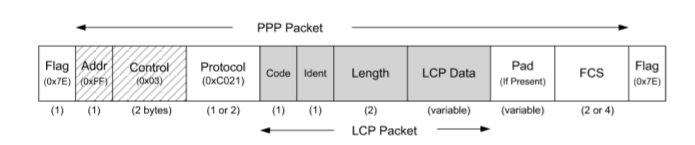
\includegraphics[width=500pt]{aufbau_ppp_frame}
  \end{center}
  \caption[Aufbau eines PPP-Frames]{Aufbau eines PPP-Frames \cite{tcpipillustrated}}
  \label{abb:aufbau_ppp_frame}
 \end{figure}

Diverse oben genannte Felder können in ihrer Länge variieren, da 
diese während des Verbindungsaufbaus vom \ac{LCP} ausgehandelt werden.

\paragraph{LCP Frame} Um die effizienteste Verbindungsart zu finden, benutzen PPP-Systeme
immer \ac{LCP}, welches korrekte Parameter aushandelt. LCP-Nachrichten in ausgetauschten
PPP-Frames enthalten somit alle Konfigurationsoptionen für die sich gerade aufbauende
Verbindung. Ist eine Konfiguration gefunden, die beide Knoten unterstützen folgt der
Link-Establishment-Prozess. Ist dieser erreicht müssen danach keine weiteren redundanten
Paketinformationen im Header mitgetragen werden.

Ein LCP-Frame ist wie folgt aufgebaut:
\begin{itemize}
	\item code (1 Byte) - hexadezimal - enhält den Messagetyp (als Codes spezifiziert)
	\item identifier (1 Byte) - hexadezimal - mit diesen werden Anfragen bzw. Antworten mit einzelnen LCP-Transaktionen in Verbindung gebracht
	\item length (2 Byte) - hexadezimal - beinhaltet die Länge der Nachricht (inklusive code, identifier, length, data)
	\item data (variabel) - hexadezimal - Nutzdaten
\end{itemize}

\ac{LCP} ist so entworfen, dass Hersteller ihre eigenen Optionen einsetzen können, ohne
selbige explizit über \ac{IANA} spezifizieren zu müssen. Dokumentiert ist dies in \textbf{RFC2153}.

\paragraph{Aufbauphasen} Nachfolgend werden die verschiedenen Aufbauphasen des
PPP-Protokolls erläutert. Im \Anhang{abb:aufbauphasen_pppverbindung} befindet
sich eine Abbildung, die diesen Vorgang illustriert.

%TODO: erst den Sinn der Phasen und dann wie das erzielt wird?
\textbf{Link Dead Phase:}
Quell- und Zielsystem fangen mit dieser Phase an und enden hiermit wieder.
Grundlage ist, dass außer (maximal) dem Link auf physischer Ebene,
keine Verbindung zwischen beiden Endpunkten besteht. Normalerweise
wird nach Sicherstellung des physischen Links von einer Seite der
Aufbau der Verbindung initiiert. Dies geschieht meist mit einer Form von Modem.
Nach Abschluss der Initiierung beginnt die nachfolgende Phase.

\textbf{Link Establishment Phase:}
Das initiierende System sendet eine \ac{LCP}-Nachricht an das Zielsystem,
um Optionen anzufordern, die gesetzt werden sollen. Dazu gehören
Netzwerklayer-Protokoll, Authentifizierungsmethode und andere optionale
Funktionen. Sofern das Zielsystem alle angeforderten Optionen beherrscht,
kann dieses eine Bestätigung (\textbf{ACK}) an das Quellsystem senden.
Ist dies nicht der Fall, wird eine Anwort verfasst, die sowohl alle
\textit{nicht unterstützten} als auch alle \text{unterstützten} Optionen
enthält, damit das Quellsystem nach Empfang dieser Information eine
Verbindung initiieren kann, die in jedem Fall von beiden Seiten unterstützt
wird. Das erfolgreiche Abschließen dieser Phase führt zur nächsten Phase.

\textbf{Authentication Phase:}
Diese Phase ist optional. Ausgelöst wird sie durch das Vorhandensein einer
Authentifizierungsoption in der LCP-Konfigurationsnachricht.
Zur Auswahl stehen z.B. \ac{PAP} oder \ac{CHAP}.
Hierbei greift PAP auf Nutzername und Passwort, CHAP auf einen komplexeren Informationsaustausch
mit einem Challenge-Response-Verfahren zurück. Der Erfolg führt immer zur nächsten
Phase, aber die Reaktion bei Misserfolg des Vorgangs ist protokollabhängig.

\textbf{Link Quality Monitoring:}
Diese Phase ist wie ihr Vorgänger ebenfalls optional - ebenfalls ausgelöst durch
die gewählt Option in der LCP-Nachricht.
Hier wird aus mehreren Protokollen gewählt. Eines davon ist standardisiert:
das 'Link Quality Report Protocol'. Registriert werden unter anderem der Linktraffic
sowie Fehlermeldungen.

\textbf{Network Layer Protocol Configuration:}
Wie bereits erwähnt, unterstützt PPP  das multiplexen von Protokollen auf
Netzwerklayerebene. Für jedes einzelne, das eingesetzt wird,
führt das System einen separaten Prozess des Verbindungsaufbaus durch.
Jedes Netzwerklayerprotokoll verfügt über einen eigenes \ac{NCP} sowie \ac{IPCP}.
Vergleichbar ist dies mit dem Aufbau von \ac{LCP} - nur spezifischer.

\textbf{Link Open Phase:}
Nachdem alle individuellen Optionen und NCP-Exchanges erfolgreich durchgeführt wurden,
ist der Verbindungsaufbau komplett und Protokolldaten können jetzt über den aufgebauten
Link in beide Richtungen ausgetauscht werden.

\textbf{Link Termination Phase:}
Wird die Verbindung absichtlich (Ablauf der Session, Authentifizierungsfehler)
oder durch Fehler o.ä. getrennt, wird im Regelfall über \ac{LCP}
eine 'Terminate Request Message' versandt. Diese kann von der Gegenseite
angenommen (\textit{AKC}) werden, sofern die grundlegende Verbindung noch aktiv ist.
Beide Systeme sind dann wieder in der ursprünglich genannten 'Link Dead Phase'.
Eine Terminierung der Verbindung ist neben \ac{LCP} auch auf \ac{NCP}-Ebene möglich,
damit die PPP-Verbindung trotz 'Terminierung' bestehen bleibt.


\subsubsection[Architektur PPPoE (Schenkel)]{Architektur PPPoE}
\label{subsubsection:architecture_pppoe}
Zur Realisierung der Verbindung zwischen Authentication Center und
Endgerät wurde in diesem Projekt aufgrund der Beschaffenheit des Raspberry Pis eine
Ethernetverbindung gewählt. Dieser wird das im vorangegangenen
Abschnitt erläuterte \ac{PPP}-Protokoll zugrunde gelegt.
In Ethernetframes werden PPP-Daten als Nutzdaten gekapselt.
Diese Methode wurde auch im realen Umfeld dazu entwickelt, \acp{ISP} die
Möglichkeit zu geben, Verbindungen über Kabelmodem oder DSL in Form
von Bridged-Topologien zu realisieren. Provider bewerkstelligen
so auch die Endpunktidentifikation, Accounting und Rechnungserstellung
(beschrieben wird der Standard in RFC2516).

\paragraph{Aufbauphasen}
Diese sind im Kontext einer PPPoE-Verbindung Discovery und Session.
Beide werden nachfolgend erläutert.

\paragraph{Discovery}
Der Client verwendet PPPoE-Frames in der Discovery-Phase dazu, einen
Zugangspunkt zu finden.

Dies geschieht in den folgenden Schritten bzw. Frames:
\begin{enumerate}
\item PPPoE Active Discovery Initiation (PADI) - Ein Frame, vom Client
      gesendet an die Broadcastadresse 0xFF-FF-FF-FF-FF-FF.
      Falls vorhanden, werden weitere Parameter als Payload 
      mitgeschickt. (Codefeld:9; Session-ID:0)
\item PPPoE Active Discovery Offer (PADO) - Ein Frame, der von der
      Authentifizierungsstelle an die Unicast MAC-Adresse des
      initiierenden Client geschickt wird. Weitere Parameter wie
      Service-Name o.ä. können ebenfalls mitgeschickt
      werden. (Codefeld:7; Session-ID:0)
\item PPPoE Active Discovery Request (PADR) - Ein Frame, der vom Client
      an die Unicat MAC-Adresse der Authentifizierungsstelle geschickt
      wird. (Codefeld:25; Session-ID:0)
\item PPPoE Active Discovery Session-Confirmation (PADS) - Ein Frame,
      der von der Authentifizierungsstelle an die Unicast MAC-Adresse
      des Client geschickt wird. Er enthält alle ausgehandelten Daten
      mit der zugewiesenen Session-ID. (Codefeld:101; Session-ID:XX)
\item PPPoE Active Discovery Terminate (PADT) - Ein Frame,
      der von beiden Endpunkten geschickt werden kann. Er signalisiert
      die gewünschte Verbindungsterminierung des Absenders.
      (Codefeld:167)
\end{enumerate}

\paragraph{Session}
In der Sessionn-Phase, ist die PPPoE-Verbindung bereits erfolgreich
aufgebaut und Daten können ausgetauscht werden.
Dieser Zustand ist erreicht, sobald die Discovery-Phase
erfolgreich abgeschlossen.

\subsubsection[Roaring Penguin PPPoE (Schenkel)]{Roaring Penguin PPPoE}
Die eingesetzte Software zur Realisierung der PPPoE-Verbindung ist der
Roaring Penguin\footnote{\url{https://www.roaringpenguin.com/products/pppoe}} PPPoE-Server.

Er implementiert den PPPoE-Standard (\Verweis{subsubsection:architecture_pppoe}) auf Basis
von \textit{TCP/IP} und \textit{PPP} als eine \textit{Userland}-Anwendung.
Dementsprechend ist es nicht notwendig hierfür den Kernel zu patchen und neu zu bauen.
Ein einfaches Installieren und konfigurieren genügt.

\paragraph{pppd}
Der im Userland installierte Dienst heißt pppd. Um eine Verbindung aufzubauen,
erstellt er eine virtuelle Netzwerkschnittstelle (der Form ppp\textit{X}) und verknüpft diese
mit einem Pseudo-\ac{tty}. %TODO: Abkürzung? Was ist tty #CHECK
Typischerweise handelt es sich hier um einem seriellen Port \cite{roaringpenguinpres}).
Daten, die von diesem tty-Device empfangen werden, erscheinen durch das ppp\textit{X}-Device.

Logisch unterhalb des tty-Device wird dann über PPPoE mit einem ebenfalls durch den Server
assoziierten Ethernet-Interface kommuniziert (eth\textit{X}).

Der Informationsfluss findet somit in nachfolgender Hierarchie statt:
 \begin{figure}[htp]
  \begin{center}
   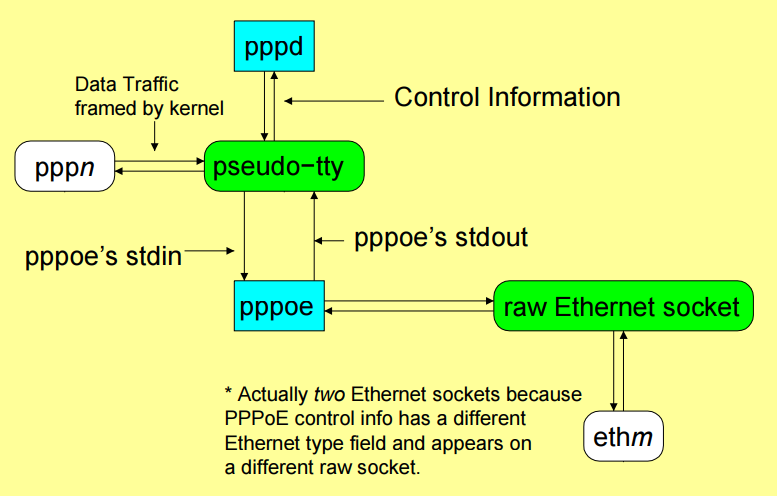
\includegraphics[width=300pt]{pppoe_roaringpenguin_2000}
  \end{center}
  \caption[Roaring Penguin PPPoE Devicehierarchie]{Roaring Penguin PPPoE Devicehierarchie \cite{roaringpenguinpres}}
  \label{fig:pppoe_roaringpenguin_devicehierarchy}
 \end{figure}

Ausgehend vom tty\textit{X}-Device kommen Daten in \ac{HDLC}-Frames zum Ethernet-Device.
Eingehende Pakete werden beim Ethernet-Device gerahmt und auf dem stdout an
das tty\textit{X}-Device weitergeleitet.

Kontroll- und Dateninformationen können bei Bedarf über unterschiedliche
Ethernet-Devices ausgetauscht werden.

%% PC/SC %%
\subsection[PC/SC (Schenkel)]{PC/SC}
Multitasking- und Multiuserbetrieb in modernen Betriebssystemen erfordert
auch das Bereitstellen eines Standards, um den Zugriff auf Chipkarten
mit mehreren (parallel arbeitenden) Teilnehmern zu organisieren. Ein Standard, der sich mit genau
dieser Problemstellung befasst ist der \textit{\ac{PC/SC}}-Standard.
Er abstrahiert die Kommunikation mit der Chipkarte so,
dass die Anwendung keine genaueren speziellen Informationen zur verwendeten
Karte benötigt. Lediglich die Kommunikation mit dem Standard
konformen Lesegerät muss durch den Treiber sichergestellt werden.

% \subsubsection{Die PC/SC-Workgroup}
Entwickelt wurde PC/SC von verschiedenen Herstellern. Hauptsächlich
Gemalto, Microsoft, Infineon und Toshiba.

\subsubsection[Spezifikation und Aufbau der Schnittstelle (Schenkel)]{Spezifikation und Aufbau der Schnittstelle}
Die Spezifikation definiert Schnittstellen, die den Zugriff auf Chipkarten ausgehend
von mehreren Applikationen beziehungsweise Nutzern ermöglichen. Grundlegend
dafür benötigt werden neben dem Standardkonformen Treiber ein \ac{IFD} und
eine \textit{PC/SC}-konforme Chipkarte (\ac{ICC} nach ISO7816-1,2 und 3).

 \begin{figure}[htp]
  \begin{center}
   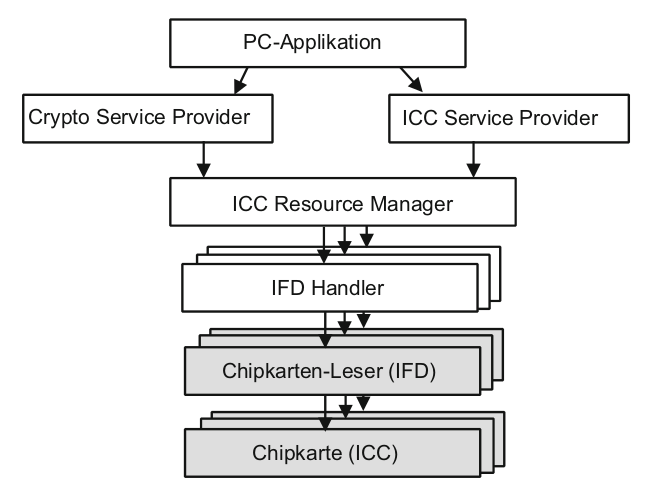
\includegraphics[width=300pt]{pcscspec_chipkartenitsicherheit}
  \end{center}
  \caption[Architektur des PC/SC-Standards]{Architektur des PC/SC-Standards \cite{spitz11}}
  \label{abb:architektur_pcsc}
 \end{figure}

Der Unterschied zum ähnlichen CT-API-Standard fängt in der Ebene
des \textit{ICC Resource Managers} an - also der Abstraktion der
APDU-Schnittstelle in der Chipkartenmiddleware \cite{spitz11}.
Selbiger Manager organisiert sowohl die Vergabe von Terminals inklusive
der vorhandenen Chipkarte, als auch das Zuordnen zusammenhängender
APDU-Kommandoketten.

Losgelöst davon können Daten auf der Chipkarte abgelegt werden. Im Umfeld
der SIM-Karte sind dies Kontakte, SMS, o.ä. Hierfür zuständig ist der
\textit{ICC Service Provider}. Ebenfalls dazu gehören administrative Dateisystemzugriffe
wie das Ändern des PIN-Codes.

Der \textit{Cryptographic Service Provider} ist die ausführende Komponente
der auf der Chipkarte implementierten Algorithmen zur Authentifizierung mittels
Kryptoalgorithmen. Auslöser für die Aufteilung in zwei Schnittstellen -
\textit{Crypto Service Provider} und \textit{ICC Service Provider} sind
rechtliche Grundlagen. In manchen Staaten ist der Import von
Verschlüsselungstechnologien auf diesem Weg untersagt.

Unter Einhaltung des Standards ist es mit oben genannter Architektur möglich,
dass parallel aus verschiedenen Anwendungen auf unterschiedliche Konstellationen
von Chipkarten und Lesern zugegriffen wird.

Sowohl unter Windows als auch in vielen Linux-Distributionen sind
\textit{PC/SC-Treiber} mittlerweile verbreitet.

\subsubsection[PCSClite (Schenkel)]{PCSClite}
Die unter Linux-Distributionen verfügbare Version ist
PCSClite\footnote{\url{https://pcsclite.alioth.debian.org/}}.
Das von David Corcoran gestartete Projekt M.U.S.C.L.E
(Movement for the Use of Smart Cards in a Linux Environment)
wird mittlerweile hauptsächlich von Ludovic Rousseau
weitergeführt\cite{pcscliteweb}.

Neben diversen Linux-Distributionen werden auch Mac OSX und diverse
BSD- sowie Unix-Derivate unterstützt.

%% Programmiersprache C %%
\subsection[Die Sprache C (Heumann)]{Die Sprache C}
 C ist eine prozedurale Programmiersprache, die nicht für einen speziellen
 Anwendungsfall entwickelt wurde. Sie hat einen hohen Verbreitungsgrad
 und ist laut \ac{IEEE} Spectrum\footnote{\url{http://spectrum.ieee.org/computing/software/the-2015-top-ten-programming-languages} [besucht am 17.05.16]}
 und RedMonk\footnote{\url{http://redmonk.com/sogrady/2016/02/19/language-rankings-1-16/} [besucht am 17.05.16]}
 unter den 10 beliebtesten Programmiersprachen. C ist eine sehr hardwarenahe
 Sprache und wird deshalb oft als Ersatz für Assembler eingesetzt. In
 diesem Kapitel soll kurz auf die Geschichte eingegangen werden, was es
 bedeutet, dass die Sprache prozedural ist und welche Besonderheiten C
 aufweist.

 \subsubsection[Geschichte (Heumann)]{Geschichte}
  Die Entwicklung von C hängt stark zusammen mit der Entwicklung des Unix-Systems.
  Dieses wurde ursprünglich in Assembler geschrieben und nun wurde
  überlegt, den Code neu zu schreiben, allerdings in B. Mit B ließen sich jedoch
  einige der Unix-Features nicht umzusetzen, wie beispielsweise die Byte-Adressierung.
  
  Deshalb wurde 1972 die Sprache C von Dennies Ritchie bei Bell Labs entwickelt. Die Portabilität war
  dabei zu Beginn nicht beabsichtigt, stattdessen war C nur für Unix-Systeme entwickelt
  worden. Allerdings wurden schnell Compiler auch auf andere Systeme portiert. 1973
  war C dann leistungsfähig genug, um den Großteil des Unix Kernels in C zu schreiben.
  
  C wurde Ende der 70er auf verschiedenen Rechensystemen, wie Mainframecomputer und
  Heimrechnern implementiert. Dies bewegte vermutlich das American National Standards
  Institude dazu, 1983 ein Komitee zu gründen, das sich um eine Standardspezifikation von
  C kümmerte. Das Komitee, X3J11, veröffentlichte 1989 seinen ersten Standard, der oft auch
  als ANSI C, Standard C oder C89 bekannt ist.
  
  Nach der Weitergabe des Standards an die \ac{ISO} 1990 wurde dieser weiterentwickelt und
  führte zu zwei weiteren Standards in 1999 (C99) und 2011 (C11). Unterstützt wird von den
  Compilern C89 und oft auch C99, wohingegen C11 nicht sehr verbreitet ist. \nocite{ritchie93}
 
 \subsubsection[Prozedurales Programmierparadigma (Heumann)]{Prozedurales Programmierparadigma}
  In der Programmierung gibt es verschiedene Stile, wie Programmcode geschrieben und strukturiert
  werden kann. Dabei gibt es einige fundamentale Stile, die als Programmierparadigmen bezeichnet
  werden. Die vier wichtigsten Paradigmen sind das imperative, funktionale, logische und objekt-
  orientierte Programmierparadigma \cite{normark03}. Das prozedurale Paradigma ist eine Spezialisierung des 
  imperativen Paradigmas. Programmiersprachen können teilweise nur mit einem Paradigma entwickelt
  werden, aber oft gibt es auch mehrere Ansätze. So kann C beispielsweise auch objekt-orientiert
  geschrieben werden, aber eigentlich gilt es als prozedurale Programmiersprache.
  
  Die Idee der prozeduralen Programmierung ist, dass Aufgaben nacheinander erledigt werden, wie
  sie aufgeschrieben sind. Im Unterschied dazu wird zum Beispiel in der objekt-orientierten
  Programmierung das Programm in Klassen aufgeteilt, welche Funktionen zur Verfügung stellen. Bei
  einer prozeduralen Sprache werden die Funktionen in Bibliotheken nach ihren Aufgabengebieten
  gruppiert und aus dem Hauptprogramm heraus abgerufen. Bei C ist dieses Programm in einer ``main''-
  Funktion enthalten, über die das Programm gestartet wird.

 \subsubsection[Besonderheiten (Heumann)]{Besonderheiten}
 C ist eine ``low-level''-Sprache, was an sich nichts Schlechtes ist, aber es bedeutet, dass C mit den
 Objekten arbeitet, mit denen auch die meisten Computern arbeiten. Konkret heißt das, dass
 C nur Zeichen, Zahlen und Speicheradressen nutzt. Durch arithmetische und logische Operationen,
 die in der Maschine implementiert sind, lassen sich diese Datentypen kombinieren und bewegen.
 Daraus resultiert, dass keine Zeichenketten wie in höheren Programmiersprachen existieren oder
 Funktionen, die auf Zeichenketten und Arrays angewendet werden können. \cite{kernighan88} \\
 Welche Besonderheiten diese Aspekte mit sich bringen, soll im Folgenden aufgezeigt werden.

 \paragraph{Pointers}
  Pointers sind Variablen, die die Speicheradressen von Variablen speichern. Sie werden in C häufig
  angewendet, da sie oft die einzige Möglichkeit sind, eine Berechnung durchzuführen und teilweise
  auch, weil sie zu kompakterem und effizienterem Code führen als andere Ansätze. \cite{kernighan88}
  Pointers sind also eine große Hilfe, aber da sie Speicheradressen speichern, sind sie auch nicht ganz
  einfach zu verwenden und können zu unerwarteten Ergebnissen führen, wenn auf eine falsche
  Speicheradresse zugegriffen wird. Wie in \Abbildung{c-pointers} dargestellt, ist in der Variable c ein
  Wert abgelegt und in der Pointervariable p ist die Adresse, in der die Variable c liegt, abgespeichert.
  
  \begin{figure}[h!]
   \begin{center}
    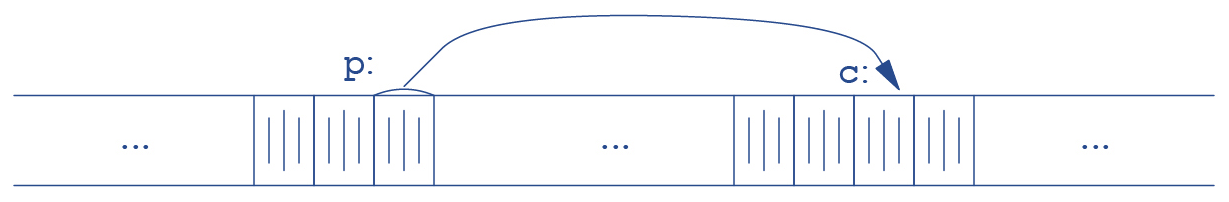
\includegraphics[width=300pt]{c-pointers}
   \end{center}
   \caption[Konzept von Pointers in C]{Konzept von Pointers \cite{kernighan88}}
   \label{fig:c-pointers}
  \end{figure}
  
  Im C-Code wird das wie folgt realisiert:

  \begin{lstlisting}[language=C]
  int c = 12;
  int* p = &c;
  \end{lstlisting}
  Durch den \emph{*} wird ein Pointer deklariert, in diesem Falle auf eine Integer-Variable. Der \&-Operator
  liefert dann die Adresse der Variable \emph{c}.

  \paragraph{Bitweise Operatoren}
  Um einzelne Bits zu manipulieren, ist es am einfachsten, mit bitweisen Operatoren zu arbeiten. In vielen
  Sprachen existieren Möglichkeiten, um diese durchzuführen, aber sie werden selten genutzt. Der Grund
  dafür ist, dass in der Regel keine einzelnen Bits manipuliert werden müssen, um eine gegebene Aufgabe
  zu erledigen. Da es in C aber nur wenige Funktionen gibt, sind sie in den meisten Programmen zwingend
  erforderlich. Es werden die sechs Operationen Und (\&), Oder ($|$), Exklusiv-Oder ($^{\wedge}$), Verschiebung nach
  links ($<<$) oder rechts ($>>$) und das Komplement ($\sim$) von C unterstützt.

  \paragraph{Bibliotheken}
  Zum Schluss soll noch etwas zu den Bibliotheken gesagt werden. In prozeduralen Sprachen lassen sich
  Funktionen in Bibliotheken bündeln. Da C jedoch von Haus aus nur wenige Funktionen bereitstellt, gibt es
  nur wenige C-Programme, die ohne eine externe Bibliothek auskommen. So gibt es einige sogenannte
  Standardbibliotheken, die von der ISO und ANSI C spezifiziert wurden. Durch diese
  Bibliotheken wird der Umfang von C erweitert und abhängig vom Betriebssystem gibt es noch andere
  Bibliotheken für verschieden Anwendungsfälle. \\
  Zusätzlich zu der Tatsache, dass C viele Bibliotheken einbindet, besitzen diese typischerweise auch
  eine Header-Datei. Die Header-Datei enthält die Prototypen der Funktionen, die vom Programm genutzt
  werden können, denn auch eine Bibliothek kann Hilfsfunktionen enthalten. Diese werden dann nicht in
  der Header-Datei notiert. Neben den Funktionsprototypen enthält die Header-Datei spezielle
  Datentypen und Konstanten, die für die Verwendung der Bibliothek notwendig sind. Die Header-Datei wird
  zu Beginn eines C-Programms eingebunden und der Compiler kann auf Basis der Header-Datei eine Überprüfung
  durchführen, ob alle genutzten Funktionen seitens des Programms in einer eingebunden Bibliothek zur
  Verfügung stehen.

\subsection[Die Sprache Python (Schenkel)]{Python}
\subsubsection{Grundlagen (Schenkel)}
\textit{Python} ist eine seit 1991 frei veröffentlichte Programmiersprache. Sie zählt
zu den interpretierten Programmiersprachen. Primäre Ziele der Sprache sind zusammengefasst:
\begin{itemize}
\item Lesbarkeit
\item Kompaktheit
\end{itemize}
Somit wird neben etablierten Sprachen eine Alternative für sowohl umfangreiche Softwareprojekte
als auch kleinere Einsatzgebiete wie Skripting im Heimcomputerbereich angeboten.

\textit{Python} konzentriert sich nicht ausschließlich auf ein einziges Programmierparadigma.
Die Sprache unterstützt objektorientierte, funktionale sowie prozedurale Programmierung. Zusätzliche
Paradigmen (unter anderem auch logische) können über Erweiterungen nachgerüstet werden.
Weiterhin verfügt \textit{Python} dynamische Typisierung und automatisches Speichermanagement. Aus
diesen Gründen ist \textit{Python} vor allem auch für Einsteiger in das Thema der Programmierung
gut geeignet. Dennoch ist \textit{Python} auch aufgrund seiner hohen Flexibilität
bei erfahrenen Entwicklern verbreitet.

In vielen Linux-Distributionen gehört \textit{Python} im gewissem Umfang zur Standardinstallation.
Mit dem ausgelieferten Interpreter können (plattformübergreifend) Programme ausgeführt werden. Bei
Bedarf ist es möglich auf eine Große Anzahl von Paketen in Standardbibliotheken zuzugreifen.

In seltenen Fällen kann es auch notwendig sein, Binärcode auszuliefern, ohne den
\textit{Python}-Interpreter zu installieren. Hierfür existieren Tools von Drittanbietern,
die aus vorliegendem \textit{Python}-Code ausführbare Programme generieren. Ein Beispiel hierfür
ist \textit{py2exe}\footnote{\url{http://www.py2exe.org/}}.

\subsubsection[Motivation zur Nutzung (Schenkel)]{Motivation zur Nutzung}
Die Entscheidung für diese Programmiersprache fällt vor allem aufgrund der Tatsache, dass bereits eine
Vielzahl von Skripten aus kleineren Projekten im Bereich der Kommunikation mit \textit{SIM}-Karten
(also auf der Seite des UE) existieren. An diese Skripte kann angeschlossen werden. Nachfolgend werden die zugrunde liegenden
Skripte näher erläutert. Diese werden für die Umsetzung dieser Studienarbeit verwendet sowie
in ihrer Funktion erweitert.

\subsection[Bibliotheken (Schenkel)]{Bibliotheken}
\subsubsection{pysim (Schenkel)}
\label{subsec:pysim}
Pysim\footnote{\url{https://github.com/kevinprince/pysim}} ist ein
Python-Skript, geschrieben von Kevin Prince,
welches Operationen direkt auf der SIM-Karte implementiert:
von Kryptoalgorithmen (wie  z.B. Milenage) über administrative Dateisystemzugriffe
bis hin zur Verwaltung von Telefonbuch, SMS oder ähnlichem.
Unterstützt wird der GSM-Authentifizierungsvorgang.

Pysim kennt verschiedene Modi und nimmt dementsprechend unterschiedliche
Parameter entgegen. Verfügbare Parameter sind Chipkartentyp, verwendetes
Device (im Betriebssystem /dev/ttyX) und Baudrate\cite{pysimprince}.

Über den normalen Betrieb einer SIM-Karte (also Authentifizierung, Auslesen, etc.)
ist es mit Pysim auch möglich, Werte auf programmierbaren SIM-Karten zu setzen.

Neben abgeschlossenen Skripten ist auch die interaktive Nutzung auf der
Python-Shell verwendbar.

\subsubsection[osmo-sim-auth (Schenkel)]{osmo-sim-auth}
\label{subsec:osmosim}
\textit{Osmo-sim-auth}\footnote{\url{http://openbsc.osmocom.org/trac/wiki/osmo-sim-auth}}
überschneidet sich im Unfang angebotener Funktionen mit \textit{pysim}. Hauptsächlich ist es,
genau wie \textit{pysim} eine Implementierung in Python, um den Authentifizierungsprozess
einer Chipkarte zu steuern. Es basiert ebenfalls auf der Grundlage des
\textit{PCSClite}-Treibers und der \textit{pyscard}-Library.

Ein Unterschied zwischen beiden python-Skripten stellte sich bei der
Realisierung der Kommunikation in der Praxis heraus:
Während \textit{pysim} auch die Programmierung von Chipkarten anbietet, ist
\textit{osmo-sim-auth} dazu in der Lage, über \ac{GSM}- hinaus auch
eine \ac{UMTS}-Authentifizierung zu leiten.
Der jeweilige Modus wird über Parameter übermittelt.
Dementsprechend verfügt \textit{osmo-sim-auth} auch über die Funktion der
Resynchronisation bezüglich der \ac{SQN}-Nummer\cite{osmosimweb}.

Entwickelt wird es vom Osmocom OpenBSC-Project, welches sich damit
beschäftigt, eine (A)GPL-lizenzierte Implementierung für den
GSM/3GPP-Protokollstack zu erzielen. Neben der Authentifizierung
in direkter Kommunikation mit der SIM-Karte werden auch folgende
Funktionalitäten durch das Projekt realisiert:
\ac{BSC},\ac{MSC},\ac{HLR},\ac{AuC},\ac{VLR}, und \ac{EIR}\cite{osmocombscweb}.

\subsubsection[pyscard (Schenkel)]{pyscard}
\label{pyscard}
Zur Verwendung des Tools \textit{pysim} oder \textit{osmo-sim-auth} wird eine Python-Bibliothek benötigt,
die Smartcard-Support für Python bereitstellt. Diese Bibliothek
ist pysim. Sie fungiert als Schnittstelle zwischen dem Treiber \textit{PC/SC}
beziehungsweise \textit{PCSClite} und der Python-Anwendung 
(dargestellt im \Anhang{abb:pyscard_schema}).

Implementierte Funktionen sind das Prüfen der gesteckten bzw. nicht gesteckten
Chipkarte, der darauffolgende Verbindungsaufbau sowie das Versenden und
Empfangen von APDUs in hexadezimaler Darstellung.
Nach erfolgreichem Verbindungsaufbau kann somit eine Kommunikation via
APDUs stattfinden.

Veröffentlicht wurde pyscard als freie Software unter der
\textit{GNU Lesser General Public License}.

\subsection[Ubuntu (Schenkel)]{Ubuntu}
\label{subsec:ubuntu}
Als Grundlage für die Umsetzung des Providers wird die Linuxdistribution Ubuntu\footnote{\url{http://www.ubuntu.com/}}
gewählt. In Desktop- sowie Serverumgebungen wird es zunehmend eingesetzt.
Unter anderem, da eins der Ziele des Projektes ist, eine stabile
'Out-Of-The-Box'-Installation zu liefern. Neben der intuitiven Installation und dem
Betrieb wird auch jeweils eine \textit{LTS}-Version der aktuellen Veröffentlichung angeboten.
Hierbei steht das Akronym \textit{LTS} für Long Term Support und garantiert dem Anwender eine
Updateversorgung (an Paketen) über insgesamt fünf Jahre hinweg. Ebenso kann bei
Bedarf separat technicher Support direkt von Canonical
Ltd. bezogen werden. Ubuntus initiale Veröffentlichung (Version 4.10) geht bis ins Jahr
2004 (20. Oktober) zurück und stammt von Debian GNU/Linux ab - es zeichnet sich
allerdings durch eine ebenso breite, allerdings darüber hinaus aktuellere Paketauswahl aus.

Motivation zum Einsatz von Ubuntu in der Version 14.04 LTS ist die bestehende Erfahrung
mit dieser Version in Verbindung mit dem PPPoE-Server von Roaring Penguin (Version 4.11). 

\subsection[Raspberry Pi (Schenkel)]{Raspberry Pi}

Die Hardwaregrundlage für das Endgerät bietet die Plattform eines Raspberry Pis, einem Kleincomputer.

\subsubsection[Raspberry Pi Foundation (Schenkel)]{Raspberry Pi Foundation}
Entwickelt wird der Raspberry Pi von der Raspberry Pi Foundation\footnote{\url{https://www.raspberrypi.org}}
(registriert in Großbritannien). Ziel der Organisation ist es,
seit Veröffentlichung des ersten Modells, einen kostengünstigen
Computer vorrangig für Bildungszwecke zu entwerfen. Auf diesem
Weg soll sowohl Erwachsenen als auch Kindern der Zugang zum
Programmieren oder anderen wissenschaftlichen Anwendungsgebieten
erleichtert werden.

Bisher wurden seit der initialen Veröffentlichung im Februar 2012(\cite{rasppifoundweb})
drei Generationen in unterschiedlichen Ausführungen
entwickelt. Die Bezeichnung A(+) beziehungsweise B(+) gibt Aufschluss
über die jeweilige Ausführung.

\subsubsection[Hardware Modell B (Schenkel)]{Hardware Modell B}
Das in diesem Projekt eingesetzte Modell B der ersten Generation verfügt über folgende Hardwarekomponenten:
\begin{itemize}
\item CPU - 700 MHz Singlecore ARM1176JZF-S
\item RAM - 512 MB
\item Speicherslot - SDHC
\item Grafikprozessor - Broadcom VideoCore IV
\end{itemize}

\subsubsection[Betriebssystem (Schenkel)]{Betriebssystem}
Als Betriebssystem gibt es für den Raspberry Pi eine breite Auswahl.
Neben einer Vielzahl von Media-Center-Plattformen sind auch alle
Desktop- beziehungsweise Server-Versionen gängiger Linux-Derivate verfügbar:
Arch Linux, Puppy Linux, Raspbian, openSUSE, Gentoo Linux, Ubuntu Mate,
CentOS, Slackware, ...

\paragraph{Raspbian}
Aufgrund hoher Stabilität und Verfügbarkeit aller benötigten Treiber
(u.a. dem SIM-Kartenleser) wurde die auf \textit{Debian GNU Linux}\footnote{\url{https://www.debian.org/}}
basierende Distribution \textit{Raspbian}\footnote{\url{https://www.raspbian.org/}} ausgewählt.
Sie erbt somit alle Eigenschaften des übergeordneten Debianprojekt.
So auch den Paketmanager \textit{dpkg} mit ca. 35.000 vorkompilierten
Softwarepaketen - in einigen Fällen für den Betrieb mit dem
Raspberry Pi optimiert. Nicht vorpaketierte Software kann auf dem Raspberry
Pi durch Vorhandensein einer Vielzahl von Libraries und Build-Tools
für die ARM-Architektur kompiliert werden.

Über den rein funktionalen Konsolenbetrieb hinaus, wird Raspbian standardmäßig mit den
Windowmanagern XFCE oder LXDE ausgeliefert.

Nachdem im Juni 2012(\cite{raspbianweb}) die erste
Version fertiggestellt wurde, ist Raspbian nach wie vor aktiv
in Entwicklung. Aktuell im stabilen Debian-Release \textit{Jessie}.
Selbiges wird auch zur Umsetzung des Endgerätes eingesetzt.
Die vorkompilierten Pakete stammen dementsprechend aus dem aktuellen
\textit{stable}-Zweig, der häufig vor allem im Umfeld des Serverbetriebes
anzutreffen ist. Die Ursache hierfür ist die Tatsache, dass das
Projekt Pakete erst nach einem langen Testprozess im \textit{unstable}-
sowie darauffolgenden \textit{testing-}Zweig für den \textit{stable}-Zweig
freigibt. Im Kontrast zu gängigen Desktop-Distributionen, die
im Vergleich zu Debian stärker auf Aktualität achten.

Neben den Zielen der Raspberry Pi Foundation verfolgt das Projekt
auch die Ziele des Debian/GNU-Projekts. Es ist dementsprechend unter
den \textit{Debian Free Software Guidelines}\footnote{\url{https://wiki.debian.org/DFSGLicenses}}
lizenziert und durch die Raspbian-Community unabhängig entwickelt.
  
\subsection[VirtualBox (Schenkel)]{VirtualBox}
Die eingesetzte Virtualisierungsplattform zur Simulation des Providers ist VirtualBox\footnote{\url{https://www.virtualbox.org/}}. Das Betriebssystem Ubuntu, der PPPoE-Server und weitere Software für
das Bereitstellen des Providers wird innerhalb einer virtuelle Maschine realisiert.

\subsubsection[Grundlage (Schenkel)]{Grundlage}
\textit{VirtualBox} ist ein open-source Typ-2 Hypervisor (\Verweis{subsubsec:hypervisor}), der
ursprünglich von der \textit{innotek GmbH}, gefolgt von \textit{Sun Microsystems} entwickelt wurde.
Damals noch \textit{Sun VirtualBox} genannt, wurde es von \textit{Oracle} übernommen und ist
nach wie vor frei zugänglich (nach der GNU GPL2 Lizenz) \cite{dash13}.

\textit{VirtualBox} bietet den Hypervisor für Hostplattformen, eine API und ein SDK zur
Bereitstellung von Werkzeugen für Gäste an. Es wird als Wirtsystem auf sowohl 32-Bit als auch
64-Bit für x86-Architekturen angeboten.

Nachfolgend werden die wichtigsten Komponenten zur Realisierung der VirtualBox-Umgebung
erläutert.

\paragraph{Wirtsystem} wird das Betriebssystem genannt, welches die Grundlage für den Hypervisor
liefert. Es gehört entweder selbst zum Hypervisor oder intergeriert diesen so, dass Gastsysteme
auf ihm betrieben werden können. Beide Typen werden unter \Verweis{subsubsec:hypervisor} genauer
erläutert.

\paragraph{Gastsystem} wird das Betriebssystem genannt, welches virtualisiert auf dem Hypervisor
abgebildet wird. Es spricht die abstrahierten, virtuellen Hardwarekomponenten an, als würde
es sich um ein physikalisches System handeln.

\paragraph{Virtuelle Maschine} (VM) benennt die Instanz aus abstrahierter Hardware und einem
darin installierten Gastsystem. Hier werden die virtuellen Komponenten (CPU, RAM, HDD, etc.)
definiert und dem Gastsystem bereitgestellt.

\paragraph{Gasterweiterungen} werden dazu benötigt, die Integration der Gastsysteme zu verbessern.
Diese sind von Gastsystem zu Gastsystem verschieden und müssen deshalb gesondert ausgeliefert werden.
Dazu gehören beispielsweise Treiber für die graphische Ausgabe, die Integration von Mauspuffern
oder dem Weiterleiten von USB-Geräten.

\paragraph{Softwarekomponenten} von Virtualbox sind in verschiedene Daemon-Prozesse aufgeteilt.
Nachfolgende werden diese aufgelistet und beschrieben \cite{victor10}:\vspace*{5mm}

\begin{table}
    \begin{tabularx}{\textwidth}{|l||X|}
    \hline
      \textbf{Bezeichnung} & \textbf{Beschreibung} \\
    \hline
    \hline
      vboxsrv & Der Prozess, der die Allokation aller Ressourcen verwaltet. \\
    \hline
    \hline
      VBoxSVC & Der VirtualBox-Serviceprozess. Er überwacht den laufenden Betrieb von virtuellen Maschinen \\
    \hline
    \hline
      vboxzoneaccess & Der solarisspezifische Daemon um VirtualBox-Devices von Oracle Slaris Containern aus anzusprechen. \\
    \hline
    \hline
      VBoxXPCOMIPCD & Der Prozess der (nicht auf Windows-Hostsystemen) Interprozesskommunikation abwickelt. \\
    \hline
    \hline
      VirtualBox & Der Clientdienst, der Ressourcenlimits definieren lässt und diese verwaltet. \\
    \hline
    \end{tabularx}%WIP
    \caption{Prozessarchitektur von VirtualBox}
\end{table}

\subsubsection[Hypervisor (Schenkel)]{Hypervisor}
\label{subsubsec:hypervisor}
Ein \textit{Hypervisor} oder auch \ac{VMM} ist die Softwarekomponente, die es ermöglicht,
mehrere Gastbetriebssysteme (in VMs) gleichzeitig zu betreiben.

Bei \textit{Hypervisorn} existieren zwei verschiedene Architekturen: \textit{Typ1} und
\textit{Typ2} \cite{dash13}.

\paragraph{Typ1} wird oft auch als 'bare metal'-\textit{Hypervisor} bezeichnet, da dieser direkt
auf der Hardware agiert. Auf ihm werden ohne weitere Zwischenschicht die virtuellen Maschinen
betrieben (vgl. \Anhang{abb:hypervisor_type1}).
Beispiele für einen \textit{Hypervisor} dieses Typs sind Microsoft Hyper-V\footnote{\url{https://www.microsoft.com/en-us/server-cloud/solutions/virtualization.aspx}}
oder VMware ESX(i)\footnote{\url{https://www.vmware.com/products/esxi-and-esx/overview}}.

\paragraph{Typ2} wird oft auch als 'hosted'-\textit{Hypervisor} bezeichnet, da dieser auf
einem Hostsystem (inklusive Betriebssystem) aufbaut. Es existiert also eine weitere Schicht
zwischen \textit{Hypervisor} und Hardware im Vergleich zu Typ 1 (vgl. \Anhang{abb:hypervisor_type2}).
Beispiele für einen \textit{Hypervisor} dieses Typs sind (neben Oracle VirtualBox) Microsoft
Virtual PC\footnote{\url{https://www.microsoft.com/en-us/download/details.aspx?id=3702&751be11f-ede8-5a0c-058c-2ee190a24fa6=True}} und
VMware Workstation\footnote{\url{https://www.vmware.com/products/workstation}}.

\paragraph{Ressourcenverwaltung} ist einer der wichtigsten Aspekte für virtualisierte Umgebungen.
Verschiedene Ressourcen müssen unter virtuellen Maschinen aufgeteilt werden, sodass weder für die
Teilnehmer ein Leistungseinbruch entsteht noch die Ressourcen ineffizient genutzt werden.
Eine zentrale Rolle spielen die Belegung von Prozessor-, Arbeitsspeicher-,
Swapspeicher- sowie Netzwerk-Kapazität. Um diese Ressourcen zu verwalten, existieren verschiedene
Ansätze.

Eine Methode ist, alle Ressourcen in diskrete Teile aufzuteilen und selbige einzeln den Teilnehmern
zuzuordnen. Diese Methode bietet sich beispielsweise bei Ressourcen mit endlicher Größe an
(CPU, RAM). Während die Umsetzung einfach zu realisieren ist, birgt dieser Ansatz einen Nachteil.
Auf diesem Weg werden einzelne Hardwareteile unter Umständen nicht effizient genutzt,
da sie aktuell nicht vom besitzenden Teilnehmer in Verwendung sind, jedoch persistent zugewiesen wurden.

Aus diesem Grund wurde eine weitere Methode entwickelt, die eine software-regulierte Grenze setzt.
Hier sorgen entweder Hypervisor oder Betriebssystem dafür, dass der Teilnehmer nicht mehr als
diese bestimmte zugewiesene Obergrenze der Ressourcennutzung erreicht. Verbleibende, aktuell
nicht verwendete Ressourcen können von anderen Teilnehmern beansprucht werden. Dies im Rahmen
ihrer eigenen Ressourcenobergrenze\cite{victor10}.

Die dritte verbreitete Methode ist der (auch in Betriebssystemen eingesetzte)
\textit{Fair Share Schedule (FSS)}. Solange ausreichend Kapazitäten zur Verfügung stehen,
erhält jeder Teilnehmer so viel Ressourcen, wie er anfordert. Ist die tatsächliche Gesamtgrenze der
Ressource erschöpft, erhält jeder Teilnehmer lediglich den Teil, den er als Minimum zugesichert bekam.
Diese Methode erreicht die effizienteste Ressourcenausnutzung \cite{victor10}.

Zu beachten ist, dass fehlende Arbeitsspeicherressourcen bei einem Teilnehmer sich negativer auswirken
können, als fehlende Prozessorressourcen. Während 10\% weniger Prozessorkapazität einen
Performanceverlust von ebenso 10\% bewirkt, kann 10\% weniger Arbeitsspeicher als erforderlich zu
erweitertem Paging-Aufwand führen. Dies kann unter Umständen auch andere Teilnehmer beeinflussen.
Aus diesem Grund muss auch der Speicher ausreichend restriktiv partitioniert beziehungsweise zugewiesen werden.

\paragraph{Sicherheit} und Isolation wird bei VirtualBox in erster Linie dadurch umgesetzt, dass
es, wie alle anderen Anwendungen für Endanwender auf der x86-Architektur, sich auf Ring 3 konzentriert.
Dieser Ring repräsentiert die geringste Privilegierungsstufe auf dem x86-Prozessor. Der Kernel
beispielsweise wird in Ring 0 betrieben. Dazwischen existieren zwei weitere Privilegierungsstufen.

Für jeden Teilnehmer wird ein einziger Prozess eröffnet. Jeglicher Code von virtuellen Teilnehmern
wird in diesem Rahmen in Ring 3 ausgeführt. So erreicht jede Applikation in einer virtuellen Maschine
nahezu die gleiche Performance, als würde sie nativ auf dem Host betrieben.

Abweichend wird der Kernelcode der virtuellen Maschine behandelt. Sollte keine Hardwarevirtualisierung
zur Verfügung stehen, wird dieser nicht in Ring 0 (wie vorgesehen), sondern lediglich in Ring 1
ausgeführt. Dies kann insofern problematisch sein, da Befehle existieren, die ausschließlich
in Ring 0 funktionieren oder sich auf Ring 1 abweichend verhalten. Aus diesem Grund überprüft
VirtualBox dauerhaft Ring 1 nach Befehlen dieser Art. Wird ein Befehl gefunden, der von dieser
Problematik betroffen ist, setzt VirtualBox diesen direkt in einen geeigneten Hypervisorbefehl
um.

In manchen Fällen ist VirtualBox nicht dazu in der Lage, den entsprechenden Code korrekt zu
interpretieren. Deshalb ist es unter Umständen notwendig, gewisse Befehle in einer
emulierten Umgebung auszuführen. Hierzu wird (unter Performanceeinbrüchen) Gebrauch von
\textit{QEMU} gemacht. 

Verfügt das Hostsystem jedoch über Hardwarevirtualisierung auf Prozessorebene 
(z.B. intel VT-x\footnote{\url{http://ark.intel.com/Products/VirtualizationTechnology}}),
kann entsprechender Kernelcode bis auf Ring 0 reichen und dort ordnungsgemäß ausgeführt werden.
Auf diesem Weg ist zusätzlich
ein Performancezuwachs beziehungsweise kein Performanceverlust zu verzeichnen \cite{victor10}.

\subsubsection[Motivation (Schenkel)]{Motivation}
\textit{VirtualBox} ermöglicht es auf einem Hostsystem, mehrere virtuelle Maschinen nebeneinander
zu betreiben. Unter Berücksichtigung der Tatsache, dass viele Applikationen nicht immer ihre
zur Verfügung stehenden Ressourcen (CPU, RAM, HDD, etc.) benötigen, können diese dynamisch verwaltet
werden. So ergibt sich eine effiziente Ressourcennutzung, für alle Komponenten, die ursprünglich
dedizierte Hardware erforderten und für sich alleine beanspruchten.

Darüber hinaus sind virtuelle Maschinen sehr portabel und können auf anderen Hostsystemen als
ursprünglich, gestartet und betrieben werden. Ebenso ist es möglich (virtuelle)
Hardwarekonfigurationen dynamisch anzupassen. Aus diesen Gründen eignen sich virtuelle
Maschinen sehr gut zu Test- und Entwicklungszwecken. Auch das Betreiben von Legacy-Betriebssystemen
ist in einer virtuellen Umgebung möglich. Systeme können flexibel für unterschiedliche
Situationen angepasst (oder auch isoliert) werden, ohne dabei großen Aufwand zu generieren.
Ebenso flexibel können fertig entwickelte und getestete Systeme reproduziert (provisioniert) werden.

Da die Verfasser dieser Arbeit über Ressourcen auf ihren Arbeits-PCs verfügen und \textit{VirtualBox}
kosteneffizient und vergleichbar ein Serversystem betreiben kann, wird selbiges eingesetzt.

\subsection[Projektumsetzung (Heumann)]{Projektumsetzung}
 \subsubsection[Anforderungen (Heumann)]{Anforderungen}
 Zu Beginn, und teilweise auch während des Projektes, wurden Anforderungen
 gestellt, die umgesetzt werden sollen und Grenzen gesetzt, die
 dem Projekt einen Rahmen vorgeben. Außerdem wurden Meilensteine definiert,
 um der Projektumsetzung mehr Struktur zu geben.
 
 In Kapitel \Verweis{idee-arbeit} wurde bereits angesprochen, dass hardwareseitig
 ein Raspberry Pi mit einem Kartenleser als \ac{UE} dienen soll und der Netzprovider
 auf einer virtuellen Maschine simuliert wird. Die Kommunikation der beiden Geräte
 wird über eine \ac{PPPoE}-Verbindung realisiert. Was nicht simuliert wird, ist der
 \ac{MSC}, da dafür eine weitere virtuelle Maschine aufgesetzt werden muss und die
 Funktionalität des Knotens darauf reduziert wäre, RES und XRES (vgl. Kapitel \ref{authentifizierungsvorgang})
 miteinander zu vergleichen.
 
 Der Vergleich der beiden Werte RES und XRES wird allerdings auch nicht an anderer
 Stelle umgesetzt, sondern fällt weg, ebenso wie bei der Resynchronisation der Vergleich
 von MAC-S mit XMAC-S. Beide Vergleiche werden gemacht um sicher zu stellen, dass
 der jeweils andere Kommunikationspartner nicht korrupt ist. Da in diesem Projekt eine
 PPPoE-Verbindung genutzt wird, ist sichergestellt, dass beide Partner nicht korrupt sind
 und eine Überprüfung deshalb überflüssig.
 
 Da das Kernziel eine erfolgreiche Authentifizierung ist, werden die nötigen Funktionen
 für sowohl die Synchronisation, als auch die Resynchronisation umgesetzt. Die Datenbank,
 in der der aktuelle SQN, beziehungsweise SEQ, gespeichert werden fällt jedoch weg, da
 diese bei nur einer USIM wieder zusätzlicher Aufwand bedeutet. \\
 Da es außerdem nur um die Authentifizierung geht, aber nicht die Kommunikation zwischen
 beiden Seiten, wird vom simulierten AuC kein CK oder IK generiert. \\
 Damit bleibt, dass bis auf \emph{f3} und \emph{f4}, alle Funktionen, die in Kapitel \Verweis{milenage}
 genannt wurden, korrekt umgesetzt werden sollen.
 
 Zur korrekten Umsetzung der Milenage-Funktionen gehört ebenfalls eine Eigen\-implementierung
 des AES-Algorithmus, aber nur für eine Blocklänge von 128 Bits, da der Milenage-Algorithmus
 keine anderen Blocklängen benötigt.
 
 Bei beiden Algorithmen geht es zudem nicht um Geschwindigkeit oder Ressourcenverbrauch.
 Das soll heißen, dass bei der Implementierung dieser nicht daraufhin optimiert wird, dass wenig
 Speicherplatz benötigt wird oder dass das Programm besonders schnell ist. Stattdessen ist lediglich
 wichtig, dass beide Algorithmen korrekt implementiert werden und am Ende die Werte generieren,
 die für die Eingabeparameter zu erwarten sind.
 
 \paragraph{Meilensteine} Die Meilensteine, die für das Projekt definiert wurden, lauten wie folgt:
 \begin{description}
 \item [27.10.2015] Die Grundlagen für die Authentifizierungs\-algorithmen sollen bekannt und verstanden sein
 \item [07.12.2015] Das Auslesen einer USIM soll funktionieren, alternativ soll eine USIM emuliert werden können
 \item [01.02.2016] Der virtuelle Netzbetreiber soll gemäß der Spezifikationen, für die nötigen Funktionen funktionieren
 \item [29.02.2016] Die USIM soll in den Authentifizierungsprozess eingebunden werden, also mit dem virtuellen Netzbetreiber kommunizieren
 \item [17.04.2016] Die Studienarbeit ist bis zu diesem Zeitpunkt fertig geschrieben
 \item [30.05.2016] Die Studienarbeit muss abgegeben werden
 \end{description}
 
 Durch die Meilensteine ist eine klare Struktur gegeben und es gibt einen Zeitpuffer am Ende,
 um eventuell auftretende Komplikationen und Verzögerungen ausgleichen zu können ohne den
 Erfolg des Projektes zu gefährden.

 \subsubsection[Unterstützende Tools (Heumann)]{Unterstützende Tools}
  Im Projekt werden einige Tools genutzt, die die Arbeit unterstützen und die Kommunikation
  unter den beiden Autoren vereinfachen. Trello und Git(hub) sollen hier kurz vorgestellt werden,
  da sie eine große Hilfe waren.

  \paragraph{Trello}
  Die web-basierte Projekt\-management\-software Trello wird vom US-amerikanischen Unternehmen
  ``Fog Creek Software'' betrieben. Gegründet wurde es am 13. September 2011 und erfreut sich  in
  letzter Zeit immer größerer Beliebtheit, sodass es seit Mitte 2015 auch auf Deutsch existiert. \\
  Wenn man bei Trello angemeldet ist, kann man mehreren sogenannten Boards zugeordnet sein. In
  diesen Boards gibt es dann Listen. So kann mit Trello schnell ein Scrum- oder Kanban-Board
  erstellt werden. Man ist darauf jedoch nicht festgelegt, weshalb die Software ziemlich
  nutzungsoffen ist. In den Listen lassen sich dann Karten anlegen, welche sowohl Text, als auch
  Bilder und Checklisten enthalten können.

  \paragraph{Git}
  Um den Programmcode und das Schreiben dieser Arbeit zu vereinfachen, wurde Git genutzt. Dies ist
  eine quelloffene verteilte Versionsverwaltung, die vom Linux Gründer Linus Torvalds entwickelt
  wurde. Der Grund dafür war, dass die Entwickler des Linuxkernels lange BitKeeper genutzt haben
  für die Versionsverwaltung, aber diese konnten durch eine Lizenzänderung nicht mehr genutzt werden,
  weshalb Torvalds sich entschied, seine eigene Verwaltung zu bauen, die seine Anforderungen erfüllt. \\
  Im Gegensatz zu beispielsweise Subversion, gibt es nicht einen zentralen Server, auf dem die komplette
  Historie gespeichert ist, sondern jeder Client ist auch ein Server und hält die Historie bereit. Dies
  ermöglicht dem Nutzer einige Interaktionen durchzuführen ohne an das Internet angebunden zu sein. \\
  Git hat bewiesen, dass es stabil ist, da viele größere Projekte wie Android oder Eclipse damit ihre
  Projekte entwickeln.
